% Options for packages loaded elsewhere
\PassOptionsToPackage{unicode}{hyperref}
\PassOptionsToPackage{hyphens}{url}
\PassOptionsToPackage{dvipsnames,svgnames,x11names}{xcolor}
%
\documentclass[
  12pt,
]{book}
\usepackage{amsmath,amssymb}
\usepackage{lmodern}
\usepackage{setspace}
\usepackage{iftex}
\ifPDFTeX
  \usepackage[T1]{fontenc}
  \usepackage[utf8]{inputenc}
  \usepackage{textcomp} % provide euro and other symbols
\else % if luatex or xetex
  \usepackage{unicode-math}
  \defaultfontfeatures{Scale=MatchLowercase}
  \defaultfontfeatures[\rmfamily]{Ligatures=TeX,Scale=1}
\fi
% Use upquote if available, for straight quotes in verbatim environments
\IfFileExists{upquote.sty}{\usepackage{upquote}}{}
\IfFileExists{microtype.sty}{% use microtype if available
  \usepackage[]{microtype}
  \UseMicrotypeSet[protrusion]{basicmath} % disable protrusion for tt fonts
}{}
\makeatletter
\@ifundefined{KOMAClassName}{% if non-KOMA class
  \IfFileExists{parskip.sty}{%
    \usepackage{parskip}
  }{% else
    \setlength{\parindent}{0pt}
    \setlength{\parskip}{6pt plus 2pt minus 1pt}}
}{% if KOMA class
  \KOMAoptions{parskip=half}}
\makeatother
\usepackage{xcolor}
\usepackage[top=1in,left=1in,right=1in,bottom=1in]{geometry}
\usepackage{listings}
\newcommand{\passthrough}[1]{#1}
\lstset{defaultdialect=[5.3]Lua}
\lstset{defaultdialect=[x86masm]Assembler}
\usepackage{longtable,booktabs,array}
\usepackage{calc} % for calculating minipage widths
% Correct order of tables after \paragraph or \subparagraph
\usepackage{etoolbox}
\makeatletter
\patchcmd\longtable{\par}{\if@noskipsec\mbox{}\fi\par}{}{}
\makeatother
% Allow footnotes in longtable head/foot
\IfFileExists{footnotehyper.sty}{\usepackage{footnotehyper}}{\usepackage{footnote}}
\makesavenoteenv{longtable}
\usepackage{graphicx}
\makeatletter
\def\maxwidth{\ifdim\Gin@nat@width>\linewidth\linewidth\else\Gin@nat@width\fi}
\def\maxheight{\ifdim\Gin@nat@height>\textheight\textheight\else\Gin@nat@height\fi}
\makeatother
% Scale images if necessary, so that they will not overflow the page
% margins by default, and it is still possible to overwrite the defaults
% using explicit options in \includegraphics[width, height, ...]{}
\setkeys{Gin}{width=\maxwidth,height=\maxheight,keepaspectratio}
% Set default figure placement to htbp
\makeatletter
\def\fps@figure{htbp}
\makeatother
\setlength{\emergencystretch}{3em} % prevent overfull lines
\providecommand{\tightlist}{%
  \setlength{\itemsep}{0pt}\setlength{\parskip}{0pt}}
\setcounter{secnumdepth}{5}
\newlength{\cslhangindent}
\setlength{\cslhangindent}{1.5em}
\newlength{\csllabelwidth}
\setlength{\csllabelwidth}{3em}
\newlength{\cslentryspacingunit} % times entry-spacing
\setlength{\cslentryspacingunit}{\parskip}
\newenvironment{CSLReferences}[2] % #1 hanging-ident, #2 entry spacing
 {% don't indent paragraphs
  \setlength{\parindent}{0pt}
  % turn on hanging indent if param 1 is 1
  \ifodd #1
  \let\oldpar\par
  \def\par{\hangindent=\cslhangindent\oldpar}
  \fi
  % set entry spacing
  \setlength{\parskip}{#2\cslentryspacingunit}
 }%
 {}
\usepackage{calc}
\newcommand{\CSLBlock}[1]{#1\hfill\break}
\newcommand{\CSLLeftMargin}[1]{\parbox[t]{\csllabelwidth}{#1}}
\newcommand{\CSLRightInline}[1]{\parbox[t]{\linewidth - \csllabelwidth}{#1}\break}
\newcommand{\CSLIndent}[1]{\hspace{\cslhangindent}#1}

% English
\usepackage{booktabs}
\usepackage{longtable}
\makeatletter
\def\thm@space@setup{%
  \thm@preskip=8pt plus 2pt minus 4pt
  \thm@postskip=\thm@preskip
}
\makeatother

% PDF中的R代码
% R Markdown代码块内有没有办法实现代码/注释的自动换行? https://d.cosx.org/d/422430-r-markdown
% 可多了解一下minted包,据说高亮效果不错。How to enable LaTeX shell-escape in bookdown: https://stackoverflow.com/questions/62799280/how-to-enable-latex-shell-escape-in-bookdown
\usepackage{fontspec}%字体的包
\usepackage{listings}
\usepackage{color}
\lstset{
  language=R,
  breaklines=true, % 允许自动换行
  backgroundcolor=\color{gray!12},
	%basicstyle=\ttfamily\small,
	basicstyle=\ttfamily,
	commentstyle=\color{green!60!black},
	keywordstyle=\color{magenta},
	stringstyle=\color{blue!50!red},
	showstringspaces=false,
	% captionpos=
	numbers=none, %left
	% numberstyle=\footnotesize\color{gray},
	% numbersep=10pt,
	% stepnumber=2, %左边数字的步幅
	tabsize=4,
	frame=TB %顶部和底部有两条竖线。
	% frame=tblr
	% frame=L,
	% framerule=1pt,
	% rulecolor=\color{red}
}


% \lstset{
%   language=C++,
%   keywordstyle = \color{blue}\bfseries,
%   commentstyle=\color{green},
%   tabsize = 4,
%   %backgroundcolor=\color{bg}
%   emph = {int,float,double,char},emphstyle=\color{fontdata},
%   emph ={[2]const, typedef},emphstyle = {[2]\color{red}}
% }

% 中文
% \usepackage{ctex}
% \usepackage{amsthm,mathrsfs}
% \usepackage{booktabs}
% \usepackage{longtable}
% \makeatletter
% \def\thm@space@setup{%
%   \thm@preskip=8pt plus 2pt minus 4pt
%   \thm@postskip=\thm@preskip
% }
% \makeatother
\ifLuaTeX
  \usepackage{selnolig}  % disable illegal ligatures
\fi
\IfFileExists{bookmark.sty}{\usepackage{bookmark}}{\usepackage{hyperref}}
\IfFileExists{xurl.sty}{\usepackage{xurl}}{} % add URL line breaks if available
\urlstyle{same} % disable monospaced font for URLs
\hypersetup{
  pdftitle={The Principle of R Package GSClassifier},
  pdfauthor={Weibin Huang},
  colorlinks=true,
  linkcolor={blue},
  filecolor={Maroon},
  citecolor={Blue},
  urlcolor={Blue},
  pdfcreator={LaTeX via pandoc}}

\title{The Principle of R Package GSClassifier}
\author{Weibin Huang}
\date{2022-09-20}

\begin{document}
\maketitle

{
\hypersetup{linkcolor=}
\setcounter{tocdepth}{2}
\tableofcontents
}
\setstretch{1.5}
\hypertarget{welcome}{%
\chapter*{Welcome}\label{welcome}}
\addcontentsline{toc}{chapter}{Welcome}

\hypertarget{basic-information}{%
\section*{Basic information}\label{basic-information}}
\addcontentsline{toc}{section}{Basic information}

\textbf{The Priciple of GSClassifier} is a book for users of R package \textbf{GSClassifier} who want to know the most details. If you're looking for the PDF edition, you can find it at here.

\begin{itemize}
\tightlist
\item
  \href{https://github.com/huangwb8/GSClassifier}{\textbf{GSClassifier}} is an R-based comprehensive classification tool for subtypes modeling and personalized calling based on pure transcriptomics. It could be used for precision medicine, such as cancer diagnosis.
\item
  The inspiration of \textbf{GSClassifier} come from \href{https://github.com/CRI-iAtlas/ImmuneSubtypeClassifier}{ImmuneSubtypeClassifier}, an R package for classification of PanCancer immune subtypes based on the work of Gibbs et al {[}\protect\hyperlink{ref-RN160}{1},\protect\hyperlink{ref-RN315}{2}{]}.
\item
  Lots of surprising features in \textbf{GSClassifier} as follows:

  \begin{itemize}
  \tightlist
  \item
    Optimized for just \passthrough{\lstinline!one sample!}
  \item
    Available for modeling and calling of brand-new \passthrough{\lstinline!GEPs-based subtypes!} in any diseases (cancers)
  \item
    No limitation of the amount of \passthrough{\lstinline!gene signatures!}(≥1) or \passthrough{\lstinline!subtypes!}(≥2)
  \item
    \passthrough{\lstinline!Normalization insensitive!} due to the use of the individual \passthrough{\lstinline!gene rank matrix!}
  \item
    More ensemble and repeatable modeling process
  \item
    More optimizations in the parallel computing
  \item
    New useful functions as supplements
  \end{itemize}
\item
  \textbf{ATTENTION!} In the future, there might be third-party contributors in \passthrough{\lstinline!GSClassifier!} platform, with some useful models for specific usages. If you use models provided by these people, \textbf{you had better know more details as possible}, including \textbf{designs, data sources, destinations, training scripts and limitations} of models, expecially those from studies under peer-review.
\item
  \textbf{MORE PROJECTS}:

  \begin{itemize}
  \tightlist
  \item
    \href{https://huangwb8.github.io/GSClassifier.principle/}{\textbf{The Principle of GSClassifier}}: A eBook with more details about GSClassifier package
  \item
    \href{https://github.com/huangwb8/luckyModel}{\textbf{luckyModel}}: Model ensemble for third-party lucky series, such GSClassifier
  \end{itemize}
\end{itemize}

\hypertarget{license}{%
\section*{License}\label{license}}
\addcontentsline{toc}{section}{License}

\textbf{GSClassifier} is released under the Apache-2.0 license. See \href{https://github.com/huangwb8/GSClassifier/blob/master/license.txt}{LICENSE} for details.

The technical documentation, as a whole, is licensed under a Creative Commons Attribution-NonCommercial-ShareAlike 4.0 International License.

The code contained in this book is simultaneously available under the \href{https://opensource.org/licenses/MIT}{MIT license}; this means that you are free to use it in your own packages, as long as you cite the source.

\hypertarget{installation}{%
\section*{Installation}\label{installation}}
\addcontentsline{toc}{section}{Installation}

\passthrough{\lstinline!RStudio!} is one of the best Integrated Development Environments (IDE) in R programming. If you're struggling in R-GUI, it is recommanded to turn to \href{https://www.rstudio.com/}{RStudio}.

For installation of \textbf{GSClassifier}, please run these commands in an R environment:

\begin{lstlisting}[language=R]
# Install "devtools" package
if (!requireNamespace("devtools", quietly = TRUE))
    install.packages("devtools")

# Install dependencies
if (!requireNamespace("luckyBase", quietly = TRUE))
    devtools::install_github("huangwb8/luckyBase")

# Install the "GSClassifier" package
if (!requireNamespace("GSClassifier", quietly = TRUE))
    devtools::install_github("huangwb8/GSClassifier")
\end{lstlisting}

In the future, a stable \passthrough{\lstinline!GSClassifier!} version might be sent to \href{https://cran.r-project.org/}{\passthrough{\lstinline!CRAN!}}. Still beta.

\hypertarget{mirror}{%
\section*{\texorpdfstring{\href{https://gitee.com/huangwb8/GSClassifier}{Mirror}}{Mirror}}\label{mirror}}
\addcontentsline{toc}{section}{\href{https://gitee.com/huangwb8/GSClassifier}{Mirror}}

For some special countries or regions, users could also try:

\begin{lstlisting}[language=R]
# Install dependencies
install.packages("https://gitee.com/huangwb8/luckyBase/repository/archive/Primary?format=tar.gz", repos=NULL, method="libcurl")

# Install the "GSClassifier" package
install.packages("https://gitee.com/huangwb8/GSClassifier/repository/archive/Primary?format=tar.gz", repos=NULL, method="libcurl")
\end{lstlisting}

\hypertarget{change-log}{%
\section*{Change log}\label{change-log}}
\addcontentsline{toc}{section}{Change log}

\hypertarget{version-0.1.9}{%
\subsection*{Version 0.1.9}\label{version-0.1.9}}
\addcontentsline{toc}{subsection}{Version 0.1.9}

\begin{itemize}
\tightlist
\item
  Optimize function verbose
\item
  Optimize for a routine scenario: one gene set and two subtypes
\item
  Optimize the strategy of automatic parameters selection for modeling training with R package \passthrough{\lstinline!caret!}
\item
  Interact with external models from the \href{https://github.com/huangwb8/luckyModel}{luckyModel} package
\end{itemize}

\hypertarget{version-0.1.8}{%
\subsection*{Version 0.1.8}\label{version-0.1.8}}
\addcontentsline{toc}{subsection}{Version 0.1.8}

\begin{itemize}
\tightlist
\item
  Primary public version of \passthrough{\lstinline!GSClassifier!}
\item
  Apache License, Version 2.0
\item
  Friendly wiki-based tutorial
\item
  Platform for developers
\end{itemize}

\hypertarget{todo}{%
\section*{TODO}\label{todo}}
\addcontentsline{toc}{section}{TODO}

\begin{itemize}
\tightlist
\item
  More medical fields included, such as in Pan-cancer uitility
\item
  Advanced methods (such as artificial intelligence) for enhanced robustness
\item
  Unsupervised learning for de-novo classification based on intrinsic frames of omics instead of human knowledges
\item
  Multi-omics exploration and support
\item
  More friendly characteristics for developers and contributors
\item
  Web application for newbies of R programing
\end{itemize}

\hypertarget{other-projects}{%
\section*{Other Projects}\label{other-projects}}
\addcontentsline{toc}{section}{Other Projects}

You may also be interested in:

\begin{itemize}
\item
  \textbf{``\href{https://github.com/huangwb8/GSClassifier}{GSClassifier}''} A comprehensive classification tool based on pure transcriptomics for precision medicine.
\item
  \textbf{``\href{https://github.com/huangwb8/luckyModel}{luckyModel}''} Model ensemble for third-party lucky series, such GSClassifier.
\end{itemize}

\hypertarget{the-principle-of-gsclassifier}{%
\chapter{The Principle of GSClassifier}\label{the-principle-of-gsclassifier}}

\hypertarget{packages}{%
\section{Packages}\label{packages}}

\begin{lstlisting}[language=R]

# Install "devtools" package
if (!requireNamespace("devtools", quietly = TRUE))
  install.packages("devtools")

# Install dependencies
if (!requireNamespace("luckyBase", quietly = TRUE))
  devtools::install_github("huangwb8/luckyBase")

# Install the "GSClassifier" package
if (!requireNamespace("GSClassifier", quietly = TRUE))
  devtools::install_github("huangwb8/GSClassifier")

# Install the "pacman" package
if (!requireNamespace("pacman", quietly = TRUE)){
  install.packages("pacman")
  library(pacman)
} else {
  library(pacman)
}

# Load needed packages
packages_needed <- c(
  "readxl",
  "ComplexHeatmap",
  "GSClassifier",
  "rpart",
  "tidyr",
  "reshape2",
  "ggplot2")
for(i in packages_needed){p_load(char=i)}
\end{lstlisting}

Here is the environment of R programming:

\begin{lstlisting}
# R version 4.0.3 (2020-10-10)
# Platform: x86_64-w64-mingw32/x64 (64-bit)
# Running under: Windows 10 x64 (build 18363)
# 
# Matrix products: default
# 
# locale:
# [1] LC_COLLATE=Chinese (Simplified)_China.936 
# [2] LC_CTYPE=Chinese (Simplified)_China.936   
# [3] LC_MONETARY=Chinese (Simplified)_China.936
# [4] LC_NUMERIC=C                              
# [5] LC_TIME=Chinese (Simplified)_China.936    
# 
# attached base packages:
# [1] grid      stats     graphics  grDevices utils     datasets  methods  
# [8] base     
# 
# other attached packages:
# [1] ggplot2_3.3.6        reshape2_1.4.4       tidyr_1.2.0         
# [4] rpart_4.1.16         GSClassifier_0.1.22  luckyBase_0.1.0     
# [7] ComplexHeatmap_2.4.3 readxl_1.4.0         pacman_0.5.1        
# 
# loaded via a namespace (and not attached):
#   [1] colorspace_2.0-3     ggsignif_0.6.3       rjson_0.2.21        
#   [4] ellipsis_0.3.2       class_7.3-20         rprojroot_2.0.3     
#   [7] circlize_0.4.15      GlobalOptions_0.1.2  fs_1.5.2            
#  [10] clue_0.3-57          rstudioapi_0.13      ggpubr_0.4.0        
#  [13] listenv_0.8.0        remotes_2.4.2        prodlim_2019.11.13  
#  [16] fansi_1.0.3          lubridate_1.8.0      codetools_0.2-18    
#  [19] splines_4.0.3        doParallel_1.0.17    cachem_1.0.6        
#  [22] knitr_1.30           pkgload_1.2.4        jsonlite_1.8.0      
#  [25] pROC_1.18.0          caret_6.0-92         broom_1.0.0         
#  [28] cluster_2.1.3        png_0.1-7            compiler_4.0.3      
#  [31] backports_1.4.1      assertthat_0.2.1     Matrix_1.2-18       
#  [34] fastmap_1.1.0        cli_3.3.0            htmltools_0.5.2     
#  [37] prettyunits_1.1.1    tools_4.0.3          gtable_0.3.0        
#  [40] glue_1.6.2           dplyr_1.0.9          Rcpp_1.0.8.3        
#  [43] carData_3.0-5        cellranger_1.1.0     vctrs_0.4.1         
#  [46] nlme_3.1-149         iterators_1.0.14     timeDate_3043.102   
#  [49] xfun_0.33            gower_1.0.0          stringr_1.4.0       
#  [52] globals_0.15.1       ps_1.4.0             testthat_3.1.0      
#  [55] lifecycle_1.0.1      devtools_2.4.3       rstatix_0.7.0       
#  [58] future_1.26.1        MASS_7.3-53          scales_1.2.0        
#  [61] ipred_0.9-12         parallel_4.0.3       RColorBrewer_1.1-3  
#  [64] yaml_2.3.5           memoise_2.0.1        stringi_1.7.6       
#  [67] desc_1.4.1           randomForest_4.6-14  foreach_1.5.2       
#  [70] hardhat_1.1.0        pkgbuild_1.3.1       lava_1.6.10         
#  [73] shape_1.4.6          tuneR_1.4.0          rlang_1.0.2         
#  [76] pkgconfig_2.0.3      evaluate_0.15        lattice_0.20-41     
#  [79] purrr_0.3.4          recipes_0.2.0        processx_3.7.0      
#  [82] tidyselect_1.1.2     parallelly_1.32.0    plyr_1.8.7          
#  [85] magrittr_2.0.3       bookdown_0.21        R6_2.5.1            
#  [88] generics_0.1.2       DBI_1.1.3            pillar_1.7.0        
#  [91] withr_2.5.0          survival_3.3-1       abind_1.4-5         
#  [94] nnet_7.3-17          tibble_3.1.7         future.apply_1.9.0  
#  [97] crayon_1.5.1         car_3.1-0            xgboost_1.6.0.1     
# [100] utf8_1.2.2           rmarkdown_2.14       GetoptLong_1.0.5    
# [103] usethis_2.1.3        data.table_1.14.2    callr_3.7.0         
# [106] ModelMetrics_1.2.2.2 digest_0.6.29        stats4_4.0.3        
# [109] signal_0.7-7         munsell_0.5.0        sessioninfo_1.2.2
\end{lstlisting}

\hypertarget{flowchart}{%
\section{Flowchart}\label{flowchart}}

The flowchart of \textbf{GSClassifier} is showed in Figure \ref{fig:flowchart}.

\begin{figure}

{\centering 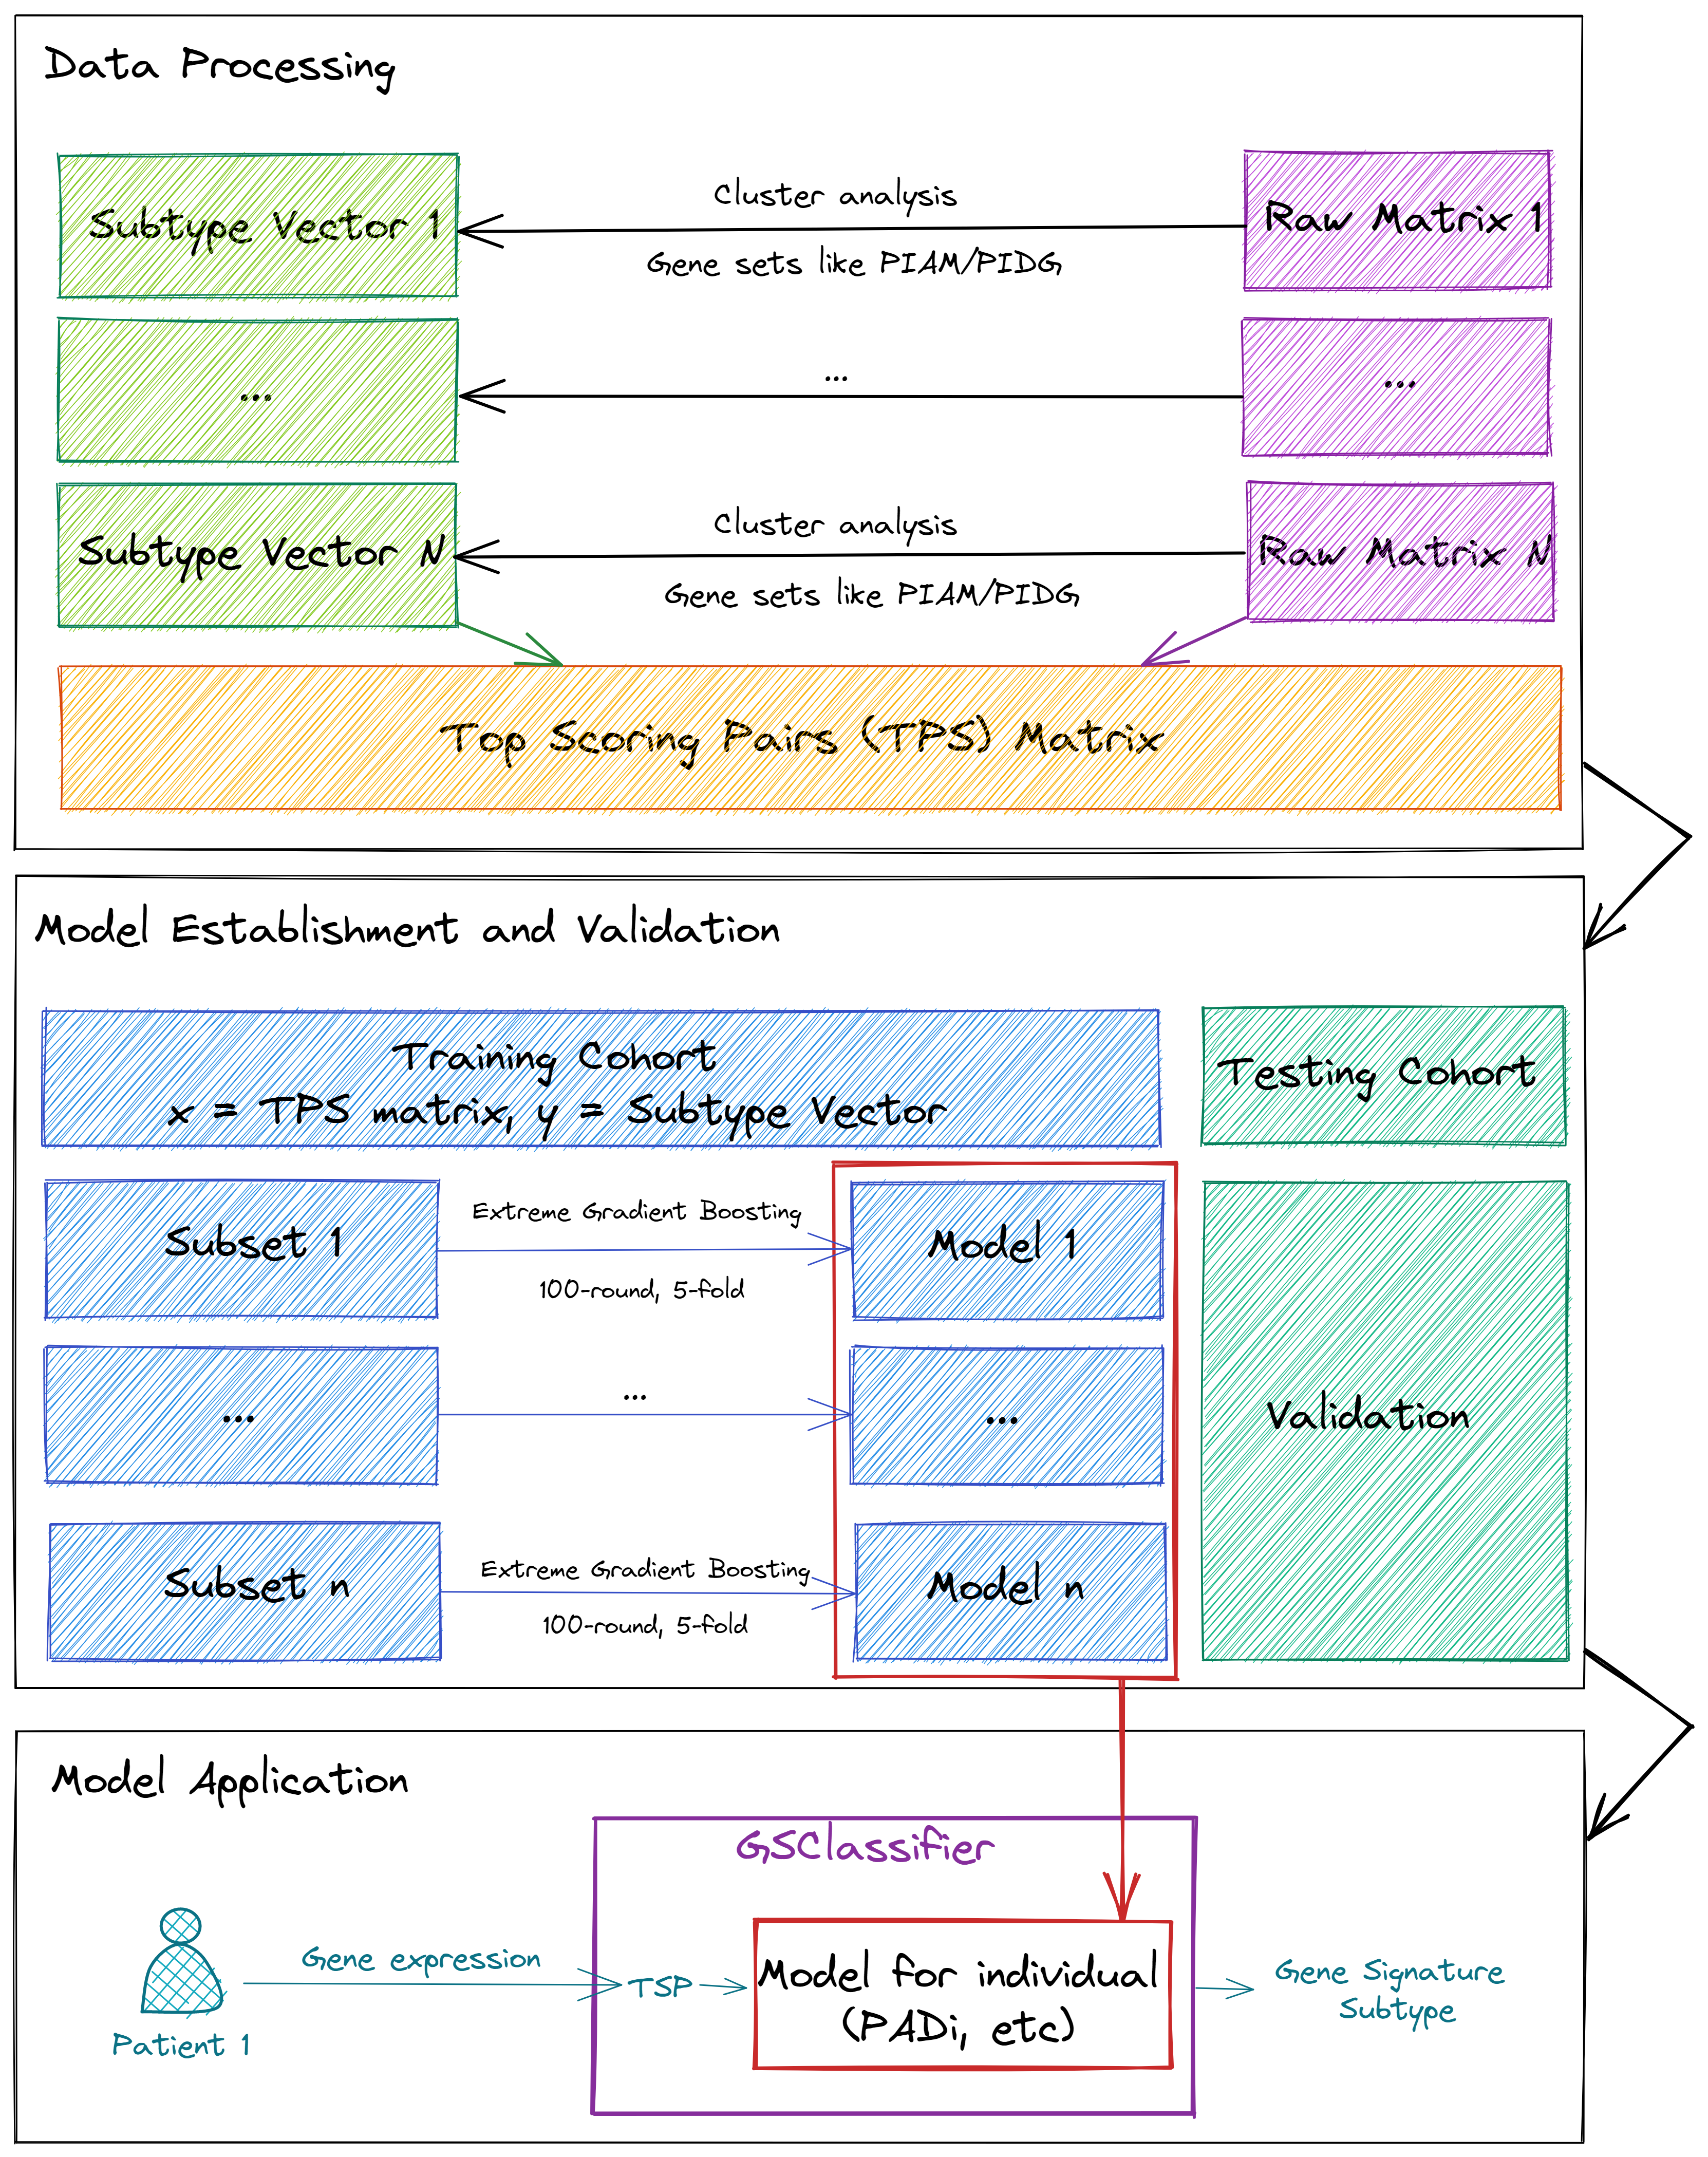
\includegraphics[width=0.9\linewidth]{./fig/flowchart} 

}

\caption{The flow chart of GSClassifier}\label{fig:flowchart}
\end{figure}

\hypertarget{data-processing}{%
\subsection{Data Processing}\label{data-processing}}

For each dataset, RNA expression matrix would be normalized internally (\textbf{Raw Matrix}) so that the expression data of the samples in the dataset were comparable and suitable for subtype identification. As demonstrated in Figure \ref{fig:flowchart}, the \textbf{Subtype vector} is identified based on independent cohorts instead of a merged matrix with batch effect control technologies. More details about batch effect control are discussed in \ref{batch-effect}.

There is no standard method to figure out subtype vectors. It depends on the Gene Expression Profiles (GEPs) used, the biological problems or ideas of researchers. For \textbf{Pan-immune Activation and Dysfunction (PAD)} subtypes, the GEPs, \textbf{Pan-Immune Activation Module (PIAM)} and \textbf{Pan-Immune Dysfunction Genes (PIDG)}, are biologically associated and suitable for calling four sutbypes (PIAM\textsuperscript{high}PIDG\textsuperscript{high}, PIAM\textsuperscript{high}PIDG\textsuperscript{low}, PIAM\textsuperscript{low}PIDG\textsuperscript{high}, and PIAM\textsuperscript{low}PIDG\textsuperscript{low}). Theoretically, we can also use a category strategy like low/medium/high, but more evidences or motivations are lacked for chasing such a complex model.

With subtype vectors and raw matrices, \textbf{Top Scoring Pairs (TSP)}, the core data format for model training and application in GSClassifier, would be calculated for the following process. The details of TSP normalization are summarized in \ref{topicTSP}.

\hypertarget{model-establishment-and-validation}{%
\subsection{Model Establishment and Validation}\label{model-establishment-and-validation}}

The TSP matrix would be devided into training cohort and internal validation cohort. In PAD project, the rate of samples (training vs.~test) is \textbf{7:3}. Next, each \textbf{SubSet} (70\% of the training cohort in PAD project) would be further selected randomly to build a \textbf{SubModel} via cross-validation Extreme Gradient Boosting algorithm (\textbf{xgboost::xgb.cv} function) {[}\protect\hyperlink{ref-RN345}{3}{]}. The number of submodels is suggested over 20 (more details in \ref{topicSubmodel}).

The internal validation cohort and external validation cohort (if any) would be used to test the performace of the trained model. By the way, \textbf{the data of both internal and external validation cohort would not be used during model training} so as to avoid over-fitting.

\hypertarget{model-application}{%
\subsection{Model Application}\label{model-application}}

In PAD project, \textbf{Model for individual}, the ensemble of submodels, is called ``PAD for individual'' (\textbf{PADi}). Supposed raw RNA expression of a sample was given. As showed in \ref{fig:flowchart} and \ref{fig:tsp}, \textbf{GSClassifier} would turn raw RNA expression into a TSP vector, which would be as a input to \textbf{Model for individual}. Then, \textbf{GSClassifier} would output the possibility matrix and the subtype for this sample. No extra data (RNA expression of others, follow-up data, etc) would be needed but RNA expression of the patient for subtype identification, so we suggest \textbf{Model for individual} (\textbf{PADi}, etc) as personalized model.

\hypertarget{topicTSP}{%
\section{Top scoring pairs}\label{topicTSP}}

\hypertarget{tsp-intro}{%
\subsection{Introduction}\label{tsp-intro}}

Genes expression of an individual is normalized during the model training and the subtype identification via \textbf{Top Scoring Pairs} (\textbf{TSP}, also called \textbf{Relative Expression Orderings} (\textbf{REOs})) algorithm, which was previously described by Geman et al {[}\protect\hyperlink{ref-RN267}{4}{]}. \textbf{TSP} normalization for an individual depends on its transcript data, implying that subtype calling would not be perturbed by data from other individuals or other extra information like follow-up data. \textbf{TSP} had been used in cancer research and effectively predicts cancer progression and ICIs response {[}\protect\hyperlink{ref-RN265}{5}--\protect\hyperlink{ref-RN261}{7}{]}.

As show in Figure \ref{fig:tsp}, The TSP data in GSClassifier consists of three parts: \textbf{binned expression}, \textbf{pair difference}, and \textbf{set difference}. In this section, we would conduct some experiments to demonstrate the potential of TSP normalization for development of cross-dataset/platform GEP-based models.

\begin{figure}

{\centering 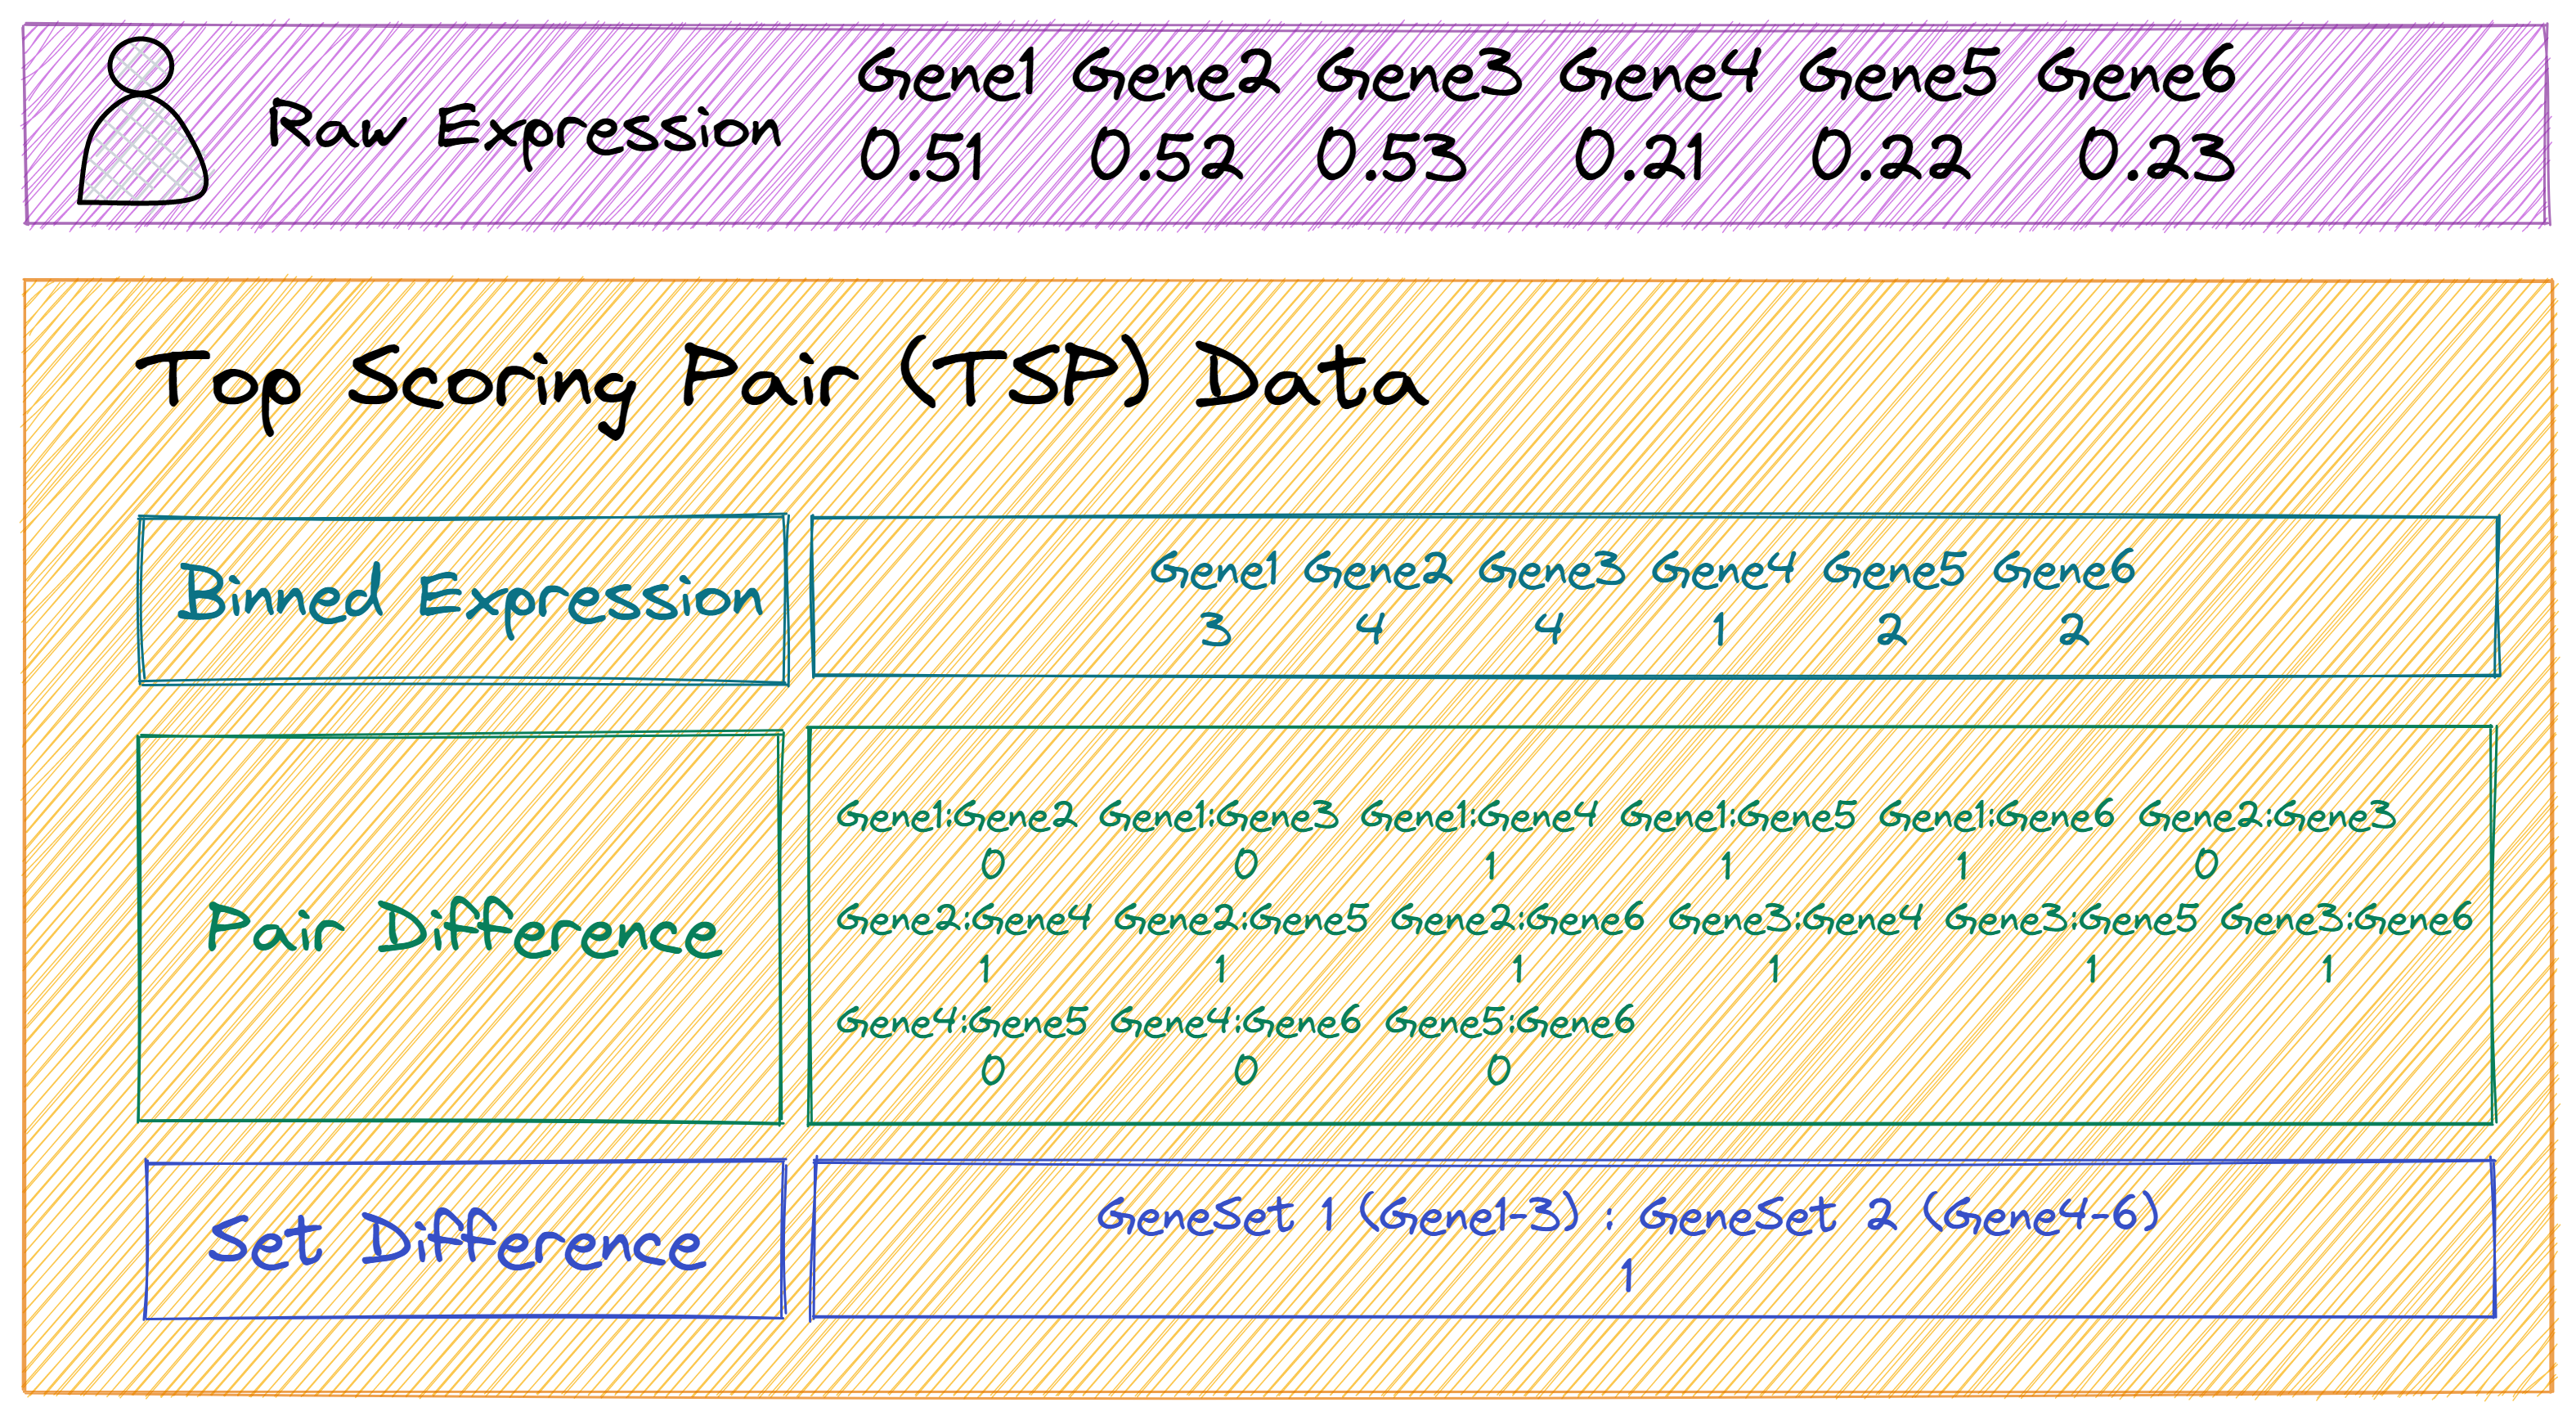
\includegraphics[width=0.85\linewidth]{./fig/TSP} 

}

\caption{The components of TSP (2 gene sets)}\label{fig:tsp}
\end{figure}

\hypertarget{simulated-dataset}{%
\subsection{Simulated Dataset}\label{simulated-dataset}}

We simulated a dataset to demonstrate TSP normalization in GSClassifier:

\begin{lstlisting}[language=R]
# Geneset
geneSet <- list(
  Set1 = paste('Gene',1:3,sep = ''),
  Set2 = paste('Gene',4:6,sep = '')
)

# RNA expression
x <- read_xlsx('./data/simulated-data.xlsx', sheet = 'RNA')
expr0 <- as.matrix(x[,-1])
rownames(expr0) <- as.character(as.matrix(x[,1])); rm(x)

# Missing value imputation (MVI)
expr <- na_fill(expr0, method = "quantile", seed = 447)
#  Missing value imputation with quantile algorithm...

# Subtype information
# It depends on the application scenarios of GEPs
subtype_vector <- c(1, 1, 1, 2, 2, 2)
# Binned data for subtype 1
Ybin <- ifelse(subtype_vector == 1, 1, 0)

# Parameters
breakVec = c(0, 0.25, 0.5, 0.75, 1.0)

# Report
cat(c('\n', 'Gene sets:', '\n'))
print(geneSet)
cat('RNA expression:', '\n')
print(expr0); cat('\n')
cat('RNA expression after MVI:', '\n')
print(expr)
# 
#  Gene sets: 
# $Set1
# [1] "Gene1" "Gene2" "Gene3"
# 
# $Set2
# [1] "Gene4" "Gene5" "Gene6"
# 
# RNA expression: 
#       Sample1 Sample2 Sample3 Sample4 Sample5 Sample6
# Gene1    0.51    0.52    0.60    0.21    0.30    0.40
# Gene2    0.52    0.54    0.58    0.22    0.31    0.35
# Gene3    0.53    0.60    0.61      NA    0.29    0.30
# Gene4    0.21    0.30    0.40    0.51    0.52    0.60
# Gene5    0.22    0.31    0.35    0.52    0.54    0.58
# Gene6    0.23    0.29    0.30    0.53      NA    0.61
# Gene7    0.10    0.12    0.09    0.11    0.12    0.14
# 
# RNA expression after MVI: 
#       Sample1 Sample2 Sample3 Sample4 Sample5 Sample6
# Gene1    0.51    0.52    0.60  0.2100 0.30000    0.40
# Gene2    0.52    0.54    0.58  0.2200 0.31000    0.35
# Gene3    0.53    0.60    0.61  0.2486 0.29000    0.30
# Gene4    0.21    0.30    0.40  0.5100 0.52000    0.60
# Gene5    0.22    0.31    0.35  0.5200 0.54000    0.58
# Gene6    0.23    0.29    0.30  0.5300 0.51774    0.61
# Gene7    0.10    0.12    0.09  0.1100 0.12000    0.14
\end{lstlisting}

Look at the matrix via heatmap:

\begin{lstlisting}[language=R]
Heatmap(t(scale(t(expr0))), name = "Z-score", column_title = "Before MVI")
\end{lstlisting}

\begin{center}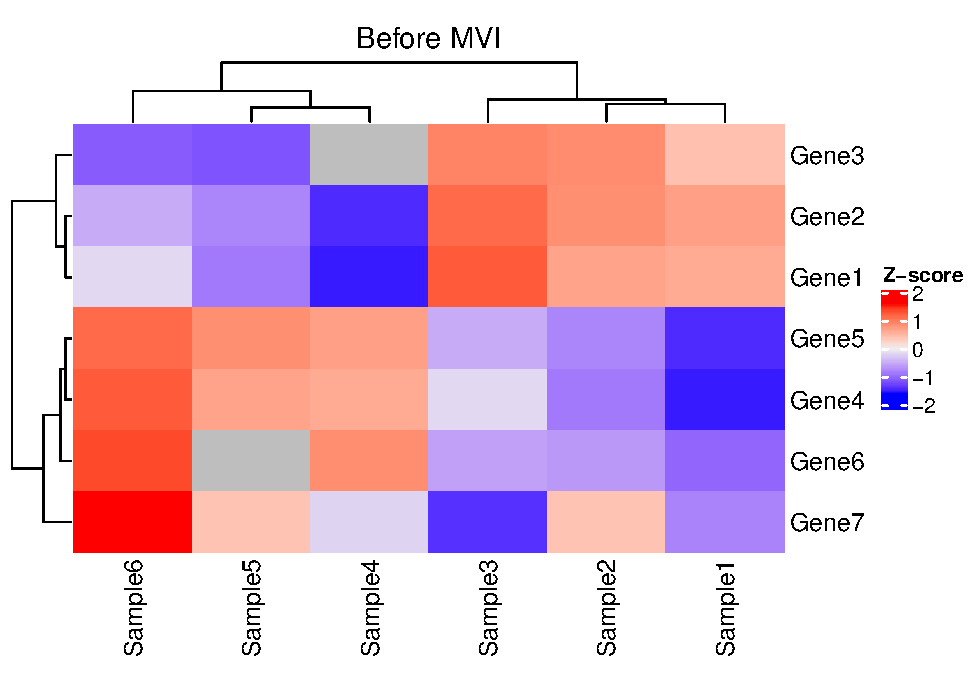
\includegraphics[width=0.6\linewidth]{Flowchart_files/figure-latex/unnamed-chunk-4-1} \end{center}

\begin{lstlisting}[language=R]
Heatmap(t(scale(t(expr))), name = "Z-score", column_title = "After MVI")
\end{lstlisting}

\begin{center}\includegraphics[width=0.6\linewidth]{Flowchart_files/figure-latex/unnamed-chunk-5-1} \end{center}

This is an intersting dataset with features as following:

\begin{itemize}
\item
  \textbf{Distinguished gene sets}: The expression profile between \textbf{Gene 1-3} and \textbf{Gene 4-6} is obviously different arross samples. Thus, these gene sets might represent different biology meaning.
\item
  \textbf{Stable gene}: The expression level and rank of \textbf{Gene 7} seemed to be similar across samples. Thus, \textbf{Gene 7} might not be a robust marker for subtype modeling. Thus, it could help us to understand how filtering of \textbf{GSClassifier} works.
\item
  \textbf{Expression heterogeneity \& rank homogeneity}: Take \textbf{Sample1} and \textbf{Sample3} as examples. The expression of \textbf{Gene 1-6} in \textbf{Sample3} seemed to be higher than those of \textbf{Sample1}. However, the expression of \textbf{Gene 1-3} is higher than \textbf{Gene 4-6} in both \textbf{Sample1} and \textbf{Sample3}, indicating similar bioprocess in these samples exists so that they should be classified as the same subtype.
\end{itemize}

\hypertarget{binned-expression}{%
\subsection{Binned expression}\label{binned-expression}}

First, we binned genes with diffrent quantile intervals so that the distribution of rank information could be more consistent across samples.

Take \textbf{Sample4} as an example:

\begin{lstlisting}[language=R]

# Data of Sample4

x <- expr[,4]

# Create quantiles  
brks <- quantile(as.numeric(x), 
                 probs=breakVec, 
                 na.rm = T)

# Get interval orders
xbin <- .bincode(x = x, 
                 breaks = brks, 
                 include.lowest = T)
xbin <- as.numeric(xbin)
names(xbin) <- names(x)

# Report
cat('Quantiles:', '\n'); print(brks)
cat('\n')
cat('Raw expression:', '\n');print(x)
cat('\n')
cat('Binned expression:', '\n'); print(xbin)
# Quantiles: 
#     0%    25%    50%    75%   100% 
# 0.1100 0.2150 0.2486 0.5150 0.5300 
# 
# Raw expression: 
#  Gene1  Gene2  Gene3  Gene4  Gene5  Gene6  Gene7 
# 0.2100 0.2200 0.2486 0.5100 0.5200 0.5300 0.1100 
# 
# Binned expression: 
# Gene1 Gene2 Gene3 Gene4 Gene5 Gene6 Gene7 
#     1     2     2     3     4     4     1
\end{lstlisting}

For example, \textbf{0.110} is the minimun of the raw expression vector, so its binned expression is \textbf{1}. Similarly, the binned expression of maximum \textbf{0.530} is \textbf{4}.

Generally, we calculate binned expression via function \textbf{breakBin} of \textbf{GSClassifier}:

\begin{lstlisting}[language=R]
expr_binned <- apply(
  expr, 2, 
  GSClassifier:::breakBin,
  breakVec)
rownames(expr_binned) <- rownames(expr)
print(expr_binned)
#       Sample1 Sample2 Sample3 Sample4 Sample5 Sample6
# Gene1       3       3       4       1       2       2
# Gene2       4       4       3       2       2       2
# Gene3       4       4       4       2       1       1
# Gene4       1       2       2       3       4       4
# Gene5       2       2       2       4       4       3
# Gene6       2       1       1       4       3       4
# Gene7       1       1       1       1       1       1
\end{lstlisting}

In this simulated dataset, \textbf{Gene7} is a gene whose expression is always the lowest across all samples. In other words, the rank of \textbf{Gene7} is stable or invariable across samples so that it's not robust for identification of differentail subtypes.

Except binned expression, we also calculated pair difference later. Due to the number of gene pair is \(C_{2 \atop n}\), the removement of genes like \textbf{Gene7} before modeling could really reduce the complexibility and save computing resources. In all, genes with low rank difference should be dropped out in some extent in \textbf{GSClassifier}.

First, We use \textbf{base::rank} to return the sample ranks of the values in a vector:

\begin{lstlisting}[language=R]
expr_binned_rank <- apply(
  expr_binned, 2, 
  function(x)rank(x, na.last = TRUE)
)
print(expr_binned_rank)
#       Sample1 Sample2 Sample3 Sample4 Sample5 Sample6
# Gene1     5.0     5.0     6.5     1.5     3.5     3.5
# Gene2     6.5     6.5     5.0     3.5     3.5     3.5
# Gene3     6.5     6.5     6.5     3.5     1.5     1.5
# Gene4     1.5     3.5     3.5     5.0     6.5     6.5
# Gene5     3.5     3.5     3.5     6.5     6.5     5.0
# Gene6     3.5     1.5     1.5     6.5     5.0     6.5
# Gene7     1.5     1.5     1.5     1.5     1.5     1.5
\end{lstlisting}

Then, get weighted average rank difference of each gene based on specified subtype distribution (\textbf{Ybin}):

\begin{lstlisting}[language=R]
testRes <- sapply(
  1:nrow(expr_binned_rank), 
  function(gi){
    
    # Rank vector of each gene
    rankg = expr_binned_rank[gi,];
    
    # Weighted average rank difference of a gene for specified subtype 
    # Here is subtype 1 vs. others
    (sum(rankg[Ybin == 0], na.rm = T) / sum(Ybin == 0, na.rm = T)) - 
    (sum(rankg[Ybin == 1], na.rm = T) / sum(Ybin == 1, na.rm = T))
  }
)
names(testRes) <- rownames(expr_binned_rank)
print(testRes)
#     Gene1     Gene2     Gene3     Gene4     Gene5     Gene6     Gene7 
# -2.666667 -2.500000 -4.333333  3.166667  2.500000  3.833333  0.000000
\end{lstlisting}

\textbf{Gene7} is the one with the lowest absolute value (0) of rank diffrence. By the way, \textbf{Gene 1-3} have the same direction (\textless0), so do \textbf{Gene 4-6} (\textgreater0), which indicates the nature of clustering based on these two gene sets.

In practice, we use \textbf{ptail} to select differential genes based on rank diffrences. \textbf{Smaller ptail is, less gene kept}. Here, we just set \textbf{ptail=0.4}:

\begin{lstlisting}[language=R]

# ptail is a numeber ranging (0,0.5].
ptail = 0.4

# Index of target genes with big rank differences
idx <- which((testRes < quantile(testRes, ptail, na.rm = T)) | 
             (testRes > quantile(testRes, 1.0-ptail, na.rm = T)))

# Target genes
gene_bigRank <- names(testRes)[idx]

# Report
cat('Index of target genes: ','\n');print(idx); cat('\n')
cat('Target genes:','\n');print(gene_bigRank)
# Index of target genes:  
# Gene1 Gene2 Gene3 Gene4 Gene5 Gene6 
#     1     2     3     4     5     6 
# 
# Target genes: 
# [1] "Gene1" "Gene2" "Gene3" "Gene4" "Gene5" "Gene6"
\end{lstlisting}

Hence, \textbf{Gene7} was filtered and excluded in the following analysis. By the way, both \textbf{ptail} and \textbf{breakVec} are hyperparameters in GSClassifier modeling.

\hypertarget{pair-difference}{%
\subsection{Pair difference}\label{pair-difference}}

In GSClassifier, we use a ensemble function \textbf{featureSelection} to select data for pair difference scoring.

\begin{lstlisting}[language=R]
expr_feat <- featureSelection(expr, Ybin,
                              testRes = testRes,
                              ptail = 0.4)

expr_sub <- expr_feat$Xsub
gene_bigRank <- expr_feat$Genes

# Report
cat('Raw xpression without NA:', '\n')
print(expr_sub)
cat('\n')
cat('Genes with large rank diff:', '\n')
print(gene_bigRank)
# Raw xpression without NA: 
#       Sample1 Sample2 Sample3 Sample4 Sample5 Sample6
# Gene1    0.51    0.52    0.60  0.2100 0.30000    0.40
# Gene2    0.52    0.54    0.58  0.2200 0.31000    0.35
# Gene3    0.53    0.60    0.61  0.2486 0.29000    0.30
# Gene4    0.21    0.30    0.40  0.5100 0.52000    0.60
# Gene5    0.22    0.31    0.35  0.5200 0.54000    0.58
# Gene6    0.23    0.29    0.30  0.5300 0.51774    0.61
# 
# Genes with large rank diff: 
# [1] "Gene1" "Gene2" "Gene3" "Gene4" "Gene5" "Gene6"
\end{lstlisting}

In GSClassifier, we use function \textbf{makeGenePairs} to calculate s

\begin{lstlisting}[language=R]
gene_bigRank_pairs <- GSClassifier:::makeGenePairs(
  gene_bigRank, 
  expr[gene_bigRank,])
print(gene_bigRank_pairs)
#             Sample1 Sample2 Sample3 Sample4 Sample5 Sample6
# Gene1:Gene2       0       0       1       0       0       1
# Gene1:Gene3       0       0       0       0       1       1
# Gene1:Gene4       1       1       1       0       0       0
# Gene1:Gene5       1       1       1       0       0       0
# Gene1:Gene6       1       1       1       0       0       0
# Gene2:Gene3       0       0       0       0       1       1
# Gene2:Gene4       1       1       1       0       0       0
# Gene2:Gene5       1       1       1       0       0       0
# Gene2:Gene6       1       1       1       0       0       0
# Gene3:Gene4       1       1       1       0       0       0
# Gene3:Gene5       1       1       1       0       0       0
# Gene3:Gene6       1       1       1       0       0       0
# Gene4:Gene5       0       0       1       0       0       1
# Gene4:Gene6       0       1       1       0       1       0
# Gene5:Gene6       0       1       1       0       1       0
\end{lstlisting}

Take \textbf{Gene1:Gene4} of \textbf{Sample1} as an example. \(Expression_{Gene1} - Expression_{Gene4} = 0.51-0.21 = 0.3 > 0\), so the pair score is 1. If the difference is less than or equal to 0, the pair score is 0. In addition, the difference of gene pair scoring between \textbf{Sample 1-3} and \textbf{Sample 4-6} is obivous, revealing the robustness of pair difference for subtype identification.

\hypertarget{set-difference}{%
\subsection{Set difference}\label{set-difference}}

In \textbf{GSClassifier}, \textbf{Set difference} is defined as a weight average of gene-geneset rank difference.

\begin{lstlisting}[language=R]
# No. of gene sets
nGS = 2

# Name of gene set comparision, which is like s1s2, s1s3 and so on.
featureNames <- 's1s2'

# Gene set difference across samples
resultList <- list()
for (i in 1:ncol(expr_sub)) { # i=1
  res0 <- numeric(length=length(featureNames))
  idx <- 1
  for (j1 in 1:(nGS-1)) { # j1=1
    for (j2 in (j1+1):nGS) { # j2=2
      
      # If j1=1 and j2=2, gene sets s1/s2 would be selected
      
      # Genes of different gene sets
      set1 <- geneSet[[j1]] # "Gene1" "Gene2" "Gene3"
      set2 <- geneSet[[j2]] # "Gene4" "Gene5" "Gene6"
      
      # RNA expression of Genes by different gene sets
      vals1 <- expr_sub[rownames(expr_sub) %in% set1,i]
      # Gene1 Gene2 Gene3
      # 0.51  0.52  0.53
      vals2 <- expr_sub[rownames(expr_sub) %in% set2,i]
      # Gene4 Gene5 Gene6
      # 0.21  0.22  0.23

      # Differences between one gene and gene sets
      # Compare expression of each gene in Set1 with all genes in Set2. 
      # For example, 0.51>0.21/0.22/0.23, so the value of Gene1:s2 is 3.
      res1 <- sapply(vals1, function(v1) sum(v1 > vals2, na.rm=T))
      # Gene1:s2   Gene2:s2   Gene3:s2
      # 3          3           3
      
      # Weight average of gene-geneset rank difference
      res0[idx] <- sum(res1, na.rm = T) / (length(vals1) * length(vals2))
      
      # Next gene set pair
      idx <- idx + 1
    }
  }
  resultList[[i]] <- as.numeric(res0)
}
resMat <- do.call(cbind, resultList)
colnames(resMat) <- colnames(expr_sub)
rownames(resMat) <- featureNames

# Report 
cat('Set difference across samples: ', '\n')
print(resMat)
# Set difference across samples:  
#      Sample1 Sample2 Sample3 Sample4 Sample5 Sample6
# s1s2       1       1       1       0       0       0
\end{lstlisting}

In \textbf{GSClassifier}, we established \textbf{makeSetData} to evaluate set difference across samples:

\begin{lstlisting}[language=R]

# Gene set difference across samples
geneset_interaction <- GSClassifier:::makeSetData(expr_sub, geneSet)

# Report 
cat('Set difference across samples: ', '\n')
print(resMat)
# Set difference across samples:  
#      Sample1 Sample2 Sample3 Sample4 Sample5 Sample6
# s1s2       1       1       1       0       0       0
\end{lstlisting}

We have known that the subtype of \textbf{Sample 1-3} differs from that of \textbf{Sample 4-6}, which revealed the robustness of set difference for subtype indentification.

Based on the structure of TSP in Figure \ref{fig:tsp}, TSP matrix of the simulated dataset should be :

\begin{lstlisting}[language=R]

# TSP matrix
tsp <- rbind(
  
  # Binned expression
  expr_binned[gene_bigRank,],
  
  # Pair difference
  gene_bigRank_pairs,
  
  # Set difference
  resMat
)

# Report 
cat('TSP matrix: ', '\n')
print(tsp)
# TSP matrix:  
#             Sample1 Sample2 Sample3 Sample4 Sample5 Sample6
# Gene1             3       3       4       1       2       2
# Gene2             4       4       3       2       2       2
# Gene3             4       4       4       2       1       1
# Gene4             1       2       2       3       4       4
# Gene5             2       2       2       4       4       3
# Gene6             2       1       1       4       3       4
# Gene1:Gene2       0       0       1       0       0       1
# Gene1:Gene3       0       0       0       0       1       1
# Gene1:Gene4       1       1       1       0       0       0
# Gene1:Gene5       1       1       1       0       0       0
# Gene1:Gene6       1       1       1       0       0       0
# Gene2:Gene3       0       0       0       0       1       1
# Gene2:Gene4       1       1       1       0       0       0
# Gene2:Gene5       1       1       1       0       0       0
# Gene2:Gene6       1       1       1       0       0       0
# Gene3:Gene4       1       1       1       0       0       0
# Gene3:Gene5       1       1       1       0       0       0
# Gene3:Gene6       1       1       1       0       0       0
# Gene4:Gene5       0       0       1       0       0       1
# Gene4:Gene6       0       1       1       0       1       0
# Gene5:Gene6       0       1       1       0       1       0
# s1s2              1       1       1       0       0       0
\end{lstlisting}

Have a look at the distribution:

\begin{lstlisting}[language=R]

# Data
tsp_df <- reshape2::melt(tsp)

ggplot(tsp_df,aes(x=Var2,y=value,fill=Var2)) + 
      geom_boxplot(outlier.size = 1, size = 1) + 
      labs(x = 'Samples',
           y = 'Epression',
           fill = NULL) 
\end{lstlisting}

\begin{center}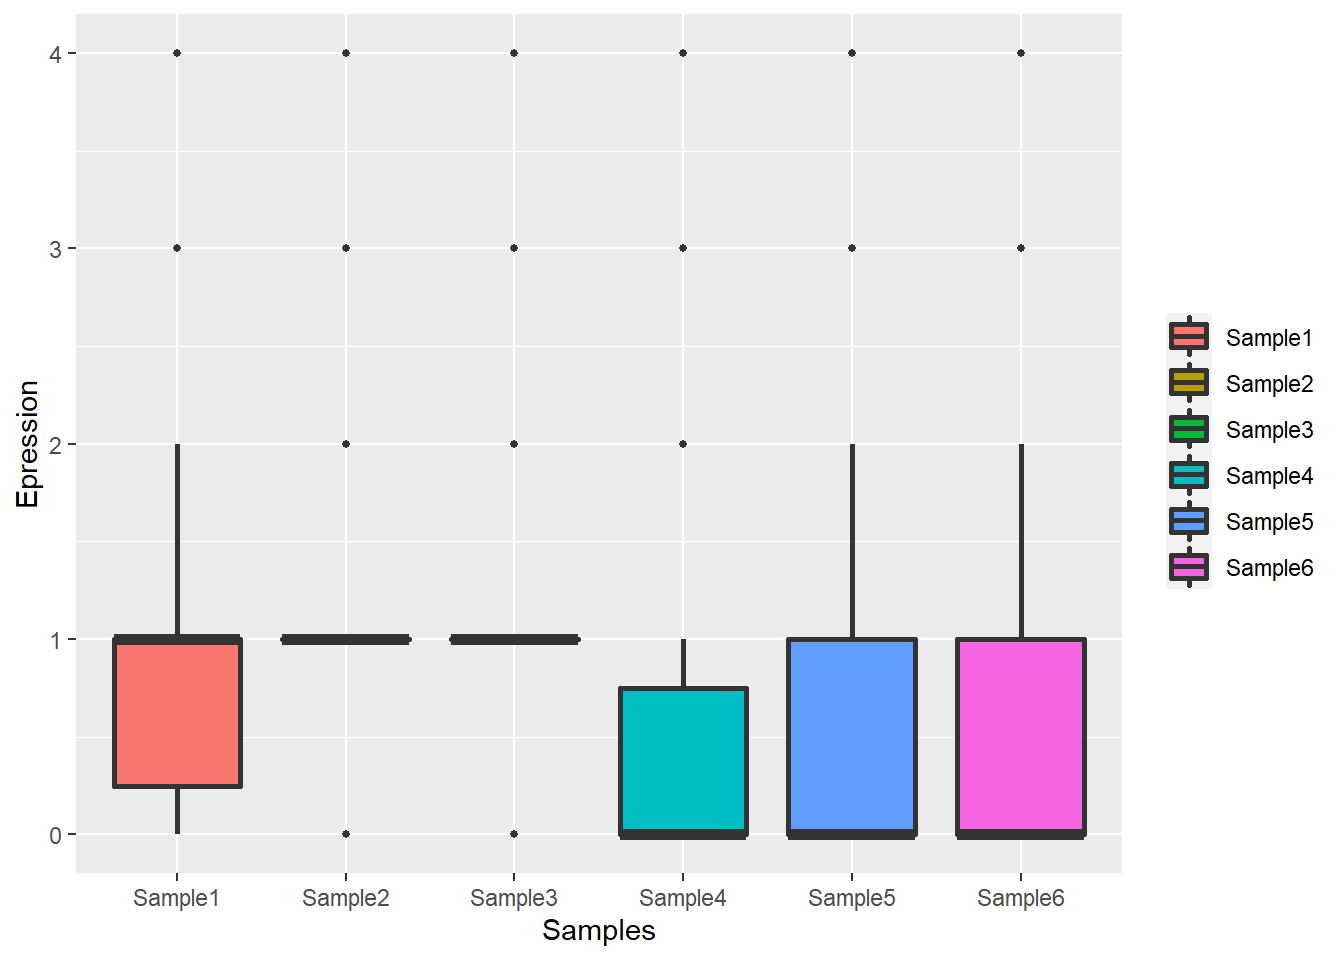
\includegraphics[width=0.6\linewidth]{Flowchart_files/figure-latex/unnamed-chunk-16-1} \end{center}

\hypertarget{discussion}{%
\chapter{Discussion}\label{discussion}}

In this section, we would discuss some key topics about \textbf{GSClassifier}, including \textbf{Missing value imputation (MVI)}, \textbf{Batch effect}, \textbf{hyperparameters}, and so on.

\hypertarget{packages-1}{%
\section{Packages}\label{packages-1}}

\begin{lstlisting}[language=R]

# Install "devtools" package
if (!requireNamespace("devtools", quietly = TRUE))
  install.packages("devtools")

# Install dependencies
if (!requireNamespace("luckyBase", quietly = TRUE))
  devtools::install_github("huangwb8/luckyBase")

# Install the "**GSClassifier**" package
if (!requireNamespace("GSClassifier", quietly = TRUE))
  devtools::install_github("huangwb8/GSClassifier")

# Install the "pacman" package
if (!requireNamespace("pacman", quietly = TRUE)){
  install.packages("pacman")
  library(pacman)
} else {
  library(pacman)
}

# Load needed packages
packages_needed <- c(
  "readxl",
  "ComplexHeatmap",
  "GSClassifier",
  "rpart",
  "tidyr",
  "reshape2",
  "ggplot2")
for(i in packages_needed){p_load(char=i)}
\end{lstlisting}

Here is the environment of R programming:

\begin{lstlisting}
# R version 4.0.3 (2020-10-10)
# Platform: x86_64-w64-mingw32/x64 (64-bit)
# Running under: Windows 10 x64 (build 18363)
# 
# Matrix products: default
# 
# locale:
# [1] LC_COLLATE=Chinese (Simplified)_China.936 
# [2] LC_CTYPE=Chinese (Simplified)_China.936   
# [3] LC_MONETARY=Chinese (Simplified)_China.936
# [4] LC_NUMERIC=C                              
# [5] LC_TIME=Chinese (Simplified)_China.936    
# 
# attached base packages:
# [1] grid      stats     graphics  grDevices utils     datasets  methods  
# [8] base     
# 
# other attached packages:
# [1] ggplot2_3.3.6        reshape2_1.4.4       tidyr_1.2.0         
# [4] rpart_4.1.16         GSClassifier_0.1.22  luckyBase_0.1.0     
# [7] ComplexHeatmap_2.4.3 readxl_1.4.0         pacman_0.5.1        
# 
# loaded via a namespace (and not attached):
#   [1] colorspace_2.0-3     ggsignif_0.6.3       rjson_0.2.21        
#   [4] ellipsis_0.3.2       class_7.3-20         rprojroot_2.0.3     
#   [7] circlize_0.4.15      GlobalOptions_0.1.2  fs_1.5.2            
#  [10] clue_0.3-57          rstudioapi_0.13      ggpubr_0.4.0        
#  [13] listenv_0.8.0        remotes_2.4.2        prodlim_2019.11.13  
#  [16] fansi_1.0.3          lubridate_1.8.0      codetools_0.2-18    
#  [19] splines_4.0.3        doParallel_1.0.17    cachem_1.0.6        
#  [22] knitr_1.30           pkgload_1.2.4        jsonlite_1.8.0      
#  [25] pROC_1.18.0          caret_6.0-92         broom_1.0.0         
#  [28] cluster_2.1.3        png_0.1-7            compiler_4.0.3      
#  [31] backports_1.4.1      assertthat_0.2.1     Matrix_1.2-18       
#  [34] fastmap_1.1.0        cli_3.3.0            htmltools_0.5.2     
#  [37] prettyunits_1.1.1    tools_4.0.3          gtable_0.3.0        
#  [40] glue_1.6.2           dplyr_1.0.9          Rcpp_1.0.8.3        
#  [43] carData_3.0-5        cellranger_1.1.0     vctrs_0.4.1         
#  [46] nlme_3.1-149         iterators_1.0.14     timeDate_3043.102   
#  [49] xfun_0.33            gower_1.0.0          stringr_1.4.0       
#  [52] globals_0.15.1       ps_1.4.0             testthat_3.1.0      
#  [55] lifecycle_1.0.1      devtools_2.4.3       rstatix_0.7.0       
#  [58] future_1.26.1        MASS_7.3-53          scales_1.2.0        
#  [61] ipred_0.9-12         parallel_4.0.3       RColorBrewer_1.1-3  
#  [64] yaml_2.3.5           memoise_2.0.1        stringi_1.7.6       
#  [67] desc_1.4.1           randomForest_4.6-14  foreach_1.5.2       
#  [70] hardhat_1.1.0        pkgbuild_1.3.1       lava_1.6.10         
#  [73] shape_1.4.6          tuneR_1.4.0          rlang_1.0.2         
#  [76] pkgconfig_2.0.3      evaluate_0.15        lattice_0.20-41     
#  [79] purrr_0.3.4          recipes_0.2.0        processx_3.7.0      
#  [82] tidyselect_1.1.2     parallelly_1.32.0    plyr_1.8.7          
#  [85] magrittr_2.0.3       bookdown_0.21        R6_2.5.1            
#  [88] generics_0.1.2       DBI_1.1.3            pillar_1.7.0        
#  [91] withr_2.5.0          survival_3.3-1       abind_1.4-5         
#  [94] nnet_7.3-17          tibble_3.1.7         future.apply_1.9.0  
#  [97] crayon_1.5.1         car_3.1-0            xgboost_1.6.0.1     
# [100] utf8_1.2.2           rmarkdown_2.14       GetoptLong_1.0.5    
# [103] usethis_2.1.3        data.table_1.14.2    callr_3.7.0         
# [106] ModelMetrics_1.2.2.2 digest_0.6.29        stats4_4.0.3        
# [109] signal_0.7-7         munsell_0.5.0        sessioninfo_1.2.2
\end{lstlisting}

\hypertarget{missing-value-imputation-mvi}{%
\section{Missing value imputation (MVI)}\label{missing-value-imputation-mvi}}

Due to reasons like low expression/weak signal, contamination of microarray surfaces, inappropriate manual operations, insufficient resolution or systematic errors during the laboratory process {[}\protect\hyperlink{ref-RN387}{8}--\protect\hyperlink{ref-RN382}{10}{]}, \textbf{missing value} in high-imput genetic data is common. Generally, tiny missing value could be just dealed with case deletion, while the biological discovery might be damaged when the missing rate tops 15\% {[}\protect\hyperlink{ref-RN392}{11},\protect\hyperlink{ref-RN386}{12}{]}. Currently, lots of methods, including statistic-based or machine learning-based methods (Figure \ref{fig:mvi01}), had been developed for \textbf{missing value imputation (MVI)} {[}\protect\hyperlink{ref-RN386}{12}{]}. Wang et al {[}\protect\hyperlink{ref-RN384}{13}{]} categorized MVI methods into simple (zeros or average),biology knowledge-, global learning-, local learning-, hybrid-based methods. In order to satisfy the working conditions of xgboost {[}\protect\hyperlink{ref-xgboost}{14}{]} functions (\passthrough{\lstinline!xgb.train!}, \passthrough{\lstinline!xgboost!}, and \passthrough{\lstinline!xgb.cv!}) in GSClassifer, the missing value in expression matrix must be deleted or imputation.

\begin{figure}

{\centering 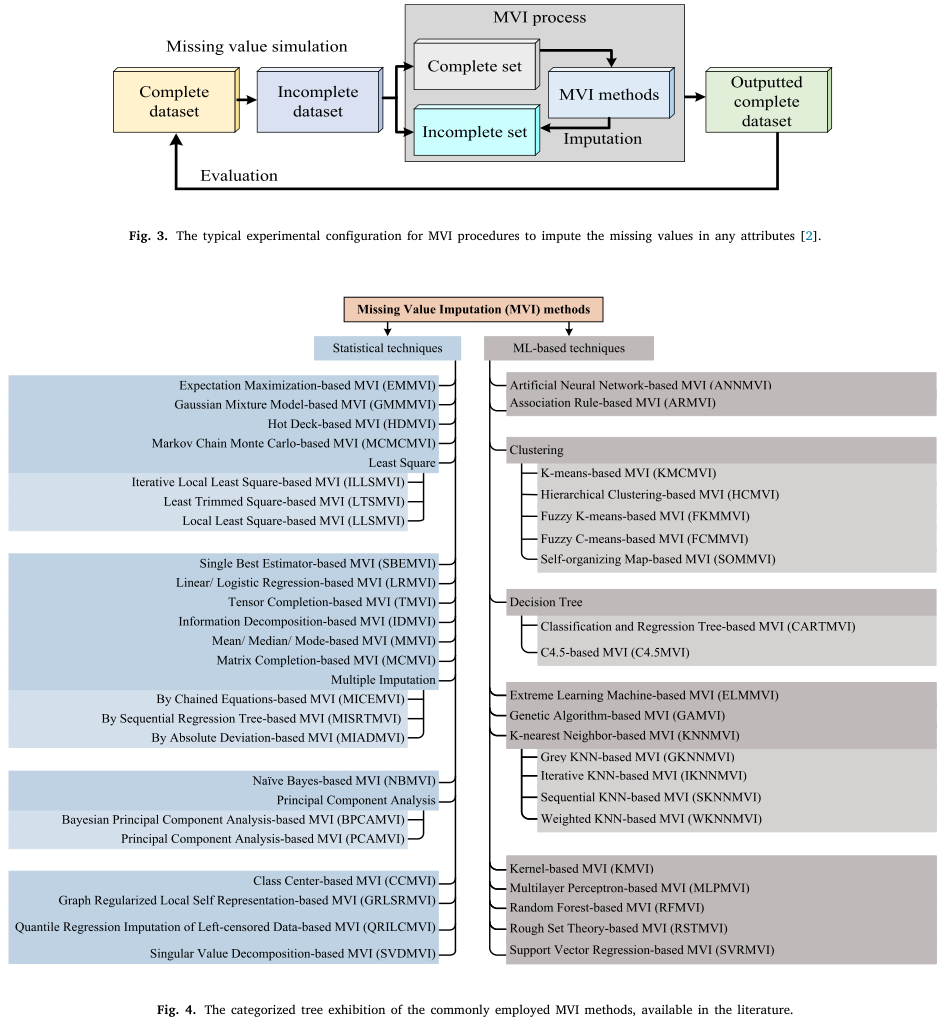
\includegraphics[width=0.9\linewidth]{./fig/mvi-01} 

}

\caption{Missing value imputation methods reviewed by Hasan et al.}\label{fig:mvi01}
\end{figure}

In \textbf{PAD} project, several strategies were applied to reduce the impact of missing values as possible. First, both \textbf{PIAM} and \textbf{PIDG} in \textbf{PAD} project were curated GEPs that were not be missing in over 80\% gastric cancer datasets. Here we showed the actual distribution of missing value across samples in gastric cancer datasets we used.

\begin{lstlisting}[language=R]
# Data
testData <- readRDS(
  system.file("extdata", 
              "testData.rds", 
              package = "GSClassifier")
  )
expr_pad <- testData$PanSTAD_expr_part

# Missing value
expr_pad_na <- apply(expr_pad, 2, 
                     function(x) sum(is.na(x))/length(x))
expr_pad_na_df <- data.frame(
  sample = names(expr_pad_na),
  prob = as.numeric(expr_pad_na),
  stringsAsFactors = F
)
\end{lstlisting}

As shown in Figure \ref{fig:mvi02}, the percentage of all samples in gastric cancer datasets we used is lower than 8\%.

\begin{lstlisting}[language=R]
# ggplot
ggplot(data = expr_pad_na_df, 
       aes(x = sample, y = prob)) + 
  geom_bar(stat = 'identity', color = mycolor[3]) + 
  scale_y_continuous(labels=scales::percent) + 
  labs(x = 'Samples in gastric cancer cohorts', 
       y = 'Percentage of missing value') + 
  theme_bw() +
  theme(
    axis.text.x = element_blank(),
    axis.ticks = element_blank(),
    axis.title = element_text(size = 15),
    axis.text = element_text(size = 12)
  )
\end{lstlisting}

\begin{figure}

{\centering 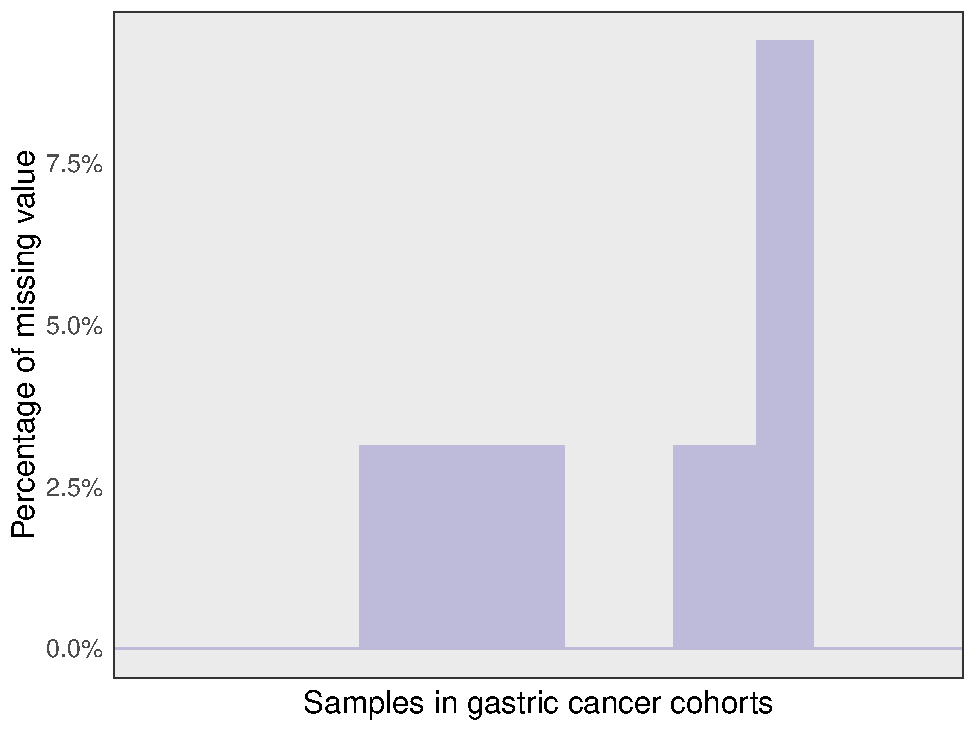
\includegraphics[width=0.8\linewidth]{Discussion_files/figure-latex/mvi02-1} 

}

\caption{The distribution of missing value across gastric cancer samples.}\label{fig:mvi02}
\end{figure}

Second, we did conduct some MVI strategy to deal with data before model training in \textbf{GSClassifier}. Due to the low missing rate of our experimental data, we just \textbf{set missing value as zero} during model training and subtype identification in the early version of PADi (\textbf{PAD.train.v20200110}). The model seemed to be robust in both the internal cohort and external cohorts, and greatly predicted the response to immune checkpoint inhibitors (ICIs) in advanced gastric cancer.

In the new version of PADi (\textbf{PAD.train.v20220917}), we designed the so-called \textbf{quantile} algorithm for random MVI during \textbf{PADi} model training, which also seemed to work well for PADi model training.

Here, we demonstrated the principle of \textbf{quantile} algorithm in the simulated dataset:

\begin{lstlisting}[language=R]
# Simulated data
x <- read_xlsx('./data/simulated-data.xlsx', sheet = 'RNA')
expr0 <- as.matrix(x[,-1])
rownames(expr0) <- as.character(as.matrix(x[,1])); rm(x)

# MVI with Quantile algorithm
expr <- expr0
na.pos <- apply(expr,2,is.one.na)
set.seed(478); seeds <- sample(1:ncol(expr)*10, sum(na.pos), replace = F)
tSample <- names(na.pos)[na.pos]
quantile_vector <- (1:1000)/1000
for(i in 1:length(tSample)){ # i=1
  
  sample.i <- tSample[i]
  expr.i <- expr[, sample.i]
  expr.i.max <- max(expr.i, na.rm = T)
  expr.i.min <- min(expr.i, na.rm = T)
  set.seed(seeds[i]);
  
  # Details of quantile algorithm
  expr.i[is.na(expr.i)] <-
    expr.i.min +
    (expr.i.max-expr.i.min) * sample(quantile_vector,
                                     sum(is.na(expr.i)),
                                     replace = T)
  expr[, sample.i] <- expr.i
}
  

# Report
cat('RNA expression:', '\n')
print(expr0)
cat('\n')
cat('RNA expression without NA value:', '\n')
print(expr)
# RNA expression: 
#       Sample1 Sample2 Sample3 Sample4 Sample5 Sample6
# Gene1    0.51    0.52    0.60    0.21    0.30    0.40
# Gene2    0.52    0.54    0.58    0.22    0.31    0.35
# Gene3    0.53    0.60    0.61      NA    0.29    0.30
# Gene4    0.21    0.30    0.40    0.51    0.52    0.60
# Gene5    0.22    0.31    0.35    0.52    0.54    0.58
# Gene6    0.23    0.29    0.30    0.53      NA    0.61
# Gene7    0.10    0.12    0.09    0.11    0.12    0.14
# 
# RNA expression without NA value: 
#       Sample1 Sample2 Sample3 Sample4 Sample5 Sample6
# Gene1    0.51    0.52    0.60 0.21000 0.30000    0.40
# Gene2    0.52    0.54    0.58 0.22000 0.31000    0.35
# Gene3    0.53    0.60    0.61 0.43256 0.29000    0.30
# Gene4    0.21    0.30    0.40 0.51000 0.52000    0.60
# Gene5    0.22    0.31    0.35 0.52000 0.54000    0.58
# Gene6    0.23    0.29    0.30 0.53000 0.32622    0.61
# Gene7    0.10    0.12    0.09 0.11000 0.12000    0.14
\end{lstlisting}

Look at the new matrix via heatmap, where the clustering result is not obviously disturbed after MVI:

\begin{lstlisting}[language=R]
Heatmap(t(scale(t(expr))), name = "Z-score", column_title = "After MVI")
\end{lstlisting}

\begin{center}\includegraphics[width=0.6\linewidth]{Discussion_files/figure-latex/unnamed-chunk-5-1} \end{center}

Due to missing value might damage the integrity of biological information, we explored \textbf{how much the number of missing value in one sample impacts subtype identification via PADi}. The steps are as following: (i) we used quantile algorithm to do MVI in the internal validation cohort of gastric cancer; (ii) we randomly masked different proportion of genes as zero expression; (iii) we calculated the relative multi-ROC {[}\protect\hyperlink{ref-pROC}{15}{]} (masked data vs.~MVI data). In \textbf{GSClassifier}, we developed a function called \textbf{mv\_tolerance} to complete the task.

\begin{enumerate}
\def\labelenumi{(\roman{enumi})}
\tightlist
\item
  Load the internal validation cohort:
\end{enumerate}

\begin{lstlisting}[language=R]
# Internal validation cohort
testData <- readRDS(
  system.file("extdata", "testData.rds", package = "GSClassifier")
  )
expr_pad <- testData$PanSTAD_expr_part
modelInfo <- modelData(
  design = testData$PanSTAD_phenotype_part,
  id.col = "ID",
  variable = c("platform", "PAD_subtype"),
  Prop = 0.7,
  seed = 19871
)
validInform <- modelInfo$Data$Valid
expr_pad_innervalid <- expr_pad[,validInform$ID]
\end{lstlisting}

\begin{enumerate}
\def\labelenumi{(\roman{enumi})}
\setcounter{enumi}{1}
\tightlist
\item
  Missing value tolerance analysis:
\end{enumerate}

\begin{lstlisting}[language=R]
# Time-consuming
mvt <- mv_tolerance(
  X = expr_pad_innervalid,
  gene.loss = c(2, 4, 6, 8, 10, 12),
  levels = c(1, 2, 3, 4),
  model = "PAD.train_20220916",
  seed = 487,
  verbose = T
)
\end{lstlisting}

\begin{enumerate}
\def\labelenumi{(\roman{enumi})}
\setcounter{enumi}{2}
\tightlist
\item
  multi-ROC analysis:
\end{enumerate}

\begin{lstlisting}[language=R]
# Data
mvt_auc <- mvt$multiAUC
mvt_auc_df <- data.frame()
for(i in 1:length(mvt_auc)){ # i=1
  df.i <- data.frame(
    x = as.integer(Fastextra(names(mvt_auc)[i], '=', 2)),
    y = as.numeric(mvt_auc[[i]]$auc),
    stringsAsFactors = F
  )
  mvt_auc_df <- rbind(mvt_auc_df, df.i)
}
  
\end{lstlisting}

\begin{lstlisting}[language=R]
ggplot(mvt_auc_df, aes(x,y)) +
  geom_point() +
  scale_x_continuous(breaks = c(2, 4, 6, 8, 10, 12)) + 
  stat_smooth(formula = y ~ x,method = 'glm') +
  labs(x = 'No. of missing value', 
       y = 'Relative AUC in multi-ROC analysis') +
  theme(
    axis.title = element_text(size = 15),
    axis.text = element_text(size = 12)
  )
\end{lstlisting}

\begin{figure}

{\centering 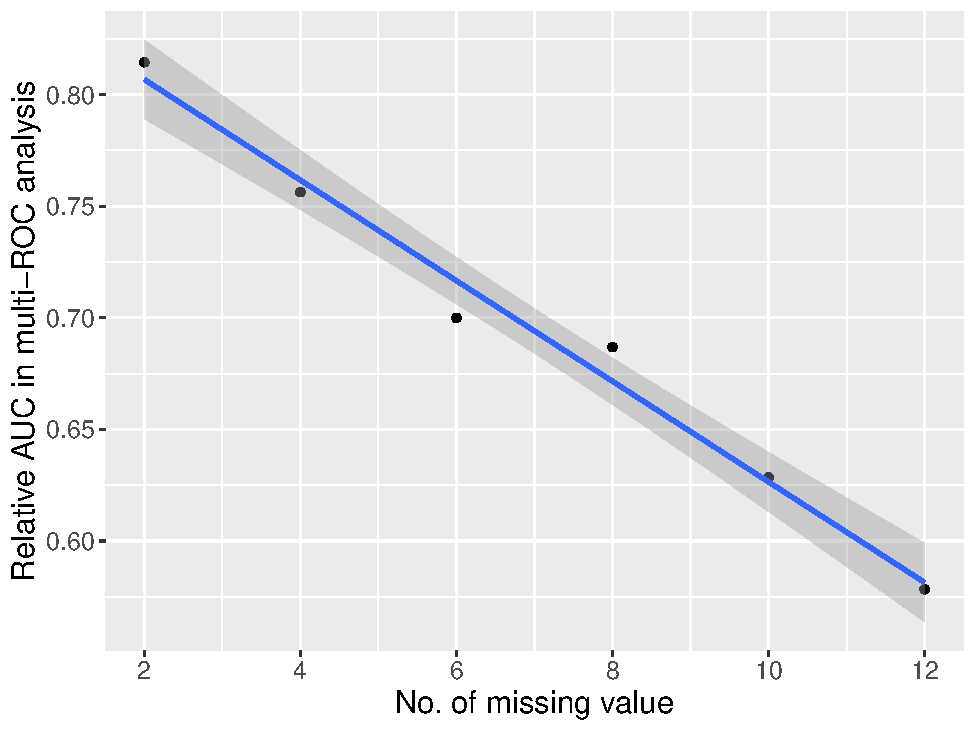
\includegraphics[width=0.6\linewidth]{Discussion_files/figure-latex/mvi03-1} 

}

\caption{The association between the number of missing value and subtype identification performance.}\label{fig:mvi03}
\end{figure}

As showed in Figure \ref{fig:mvi03}, there is linear negative correlation between the number of missing value (mising rate ranges from 6.25\% to 37.5\%) and subtype identification performance of \textbf{PADi} model. One of the reasons might be that PIAM/PIDG were small GEPs, so little gene loss might significantly impact the performance of \textbf{PADi}. By the way, there is no mising value in PIAM/PIDG of the `Kim2018' cohort, an external validation cohort for ICIs therapy response prediction via \textbf{PADi}. Nonetheless, we still used \textbf{zero strategy} during subtype identification of \textbf{PADi} if any missing value exist, because randomization might make the result unstable, which is not suitable for clinical decision.

In conclusion, zero or quantile strategy could be applied for MVI before \textbf{GSClassifier} model training. However, missing value should be avoided as possible in subtype identification for missing value really damage the performance of \textbf{GSClassifier}. Nonetheless, due to low-input GEPs used in \textbf{PADi} model (No.~of Gene=32), it's easy to avoid missing value in clinical practice.

\hypertarget{batch-effect}{%
\section{Batch effect}\label{batch-effect}}

\textbf{TSP} was widely applied to control batch effects in transciptomic data {[}\protect\hyperlink{ref-RN369}{16}--\protect\hyperlink{ref-RN365}{23}{]}. Still, we tested whether \textbf{TSP} is a robust method for batch effect control in real-world data. As demonstrated in Figure \ref{fig:be01}, the obvious batch effects across gastric cancer datsets were significantly reduced after \textbf{TSP} normalization.

\begin{figure}

{\centering 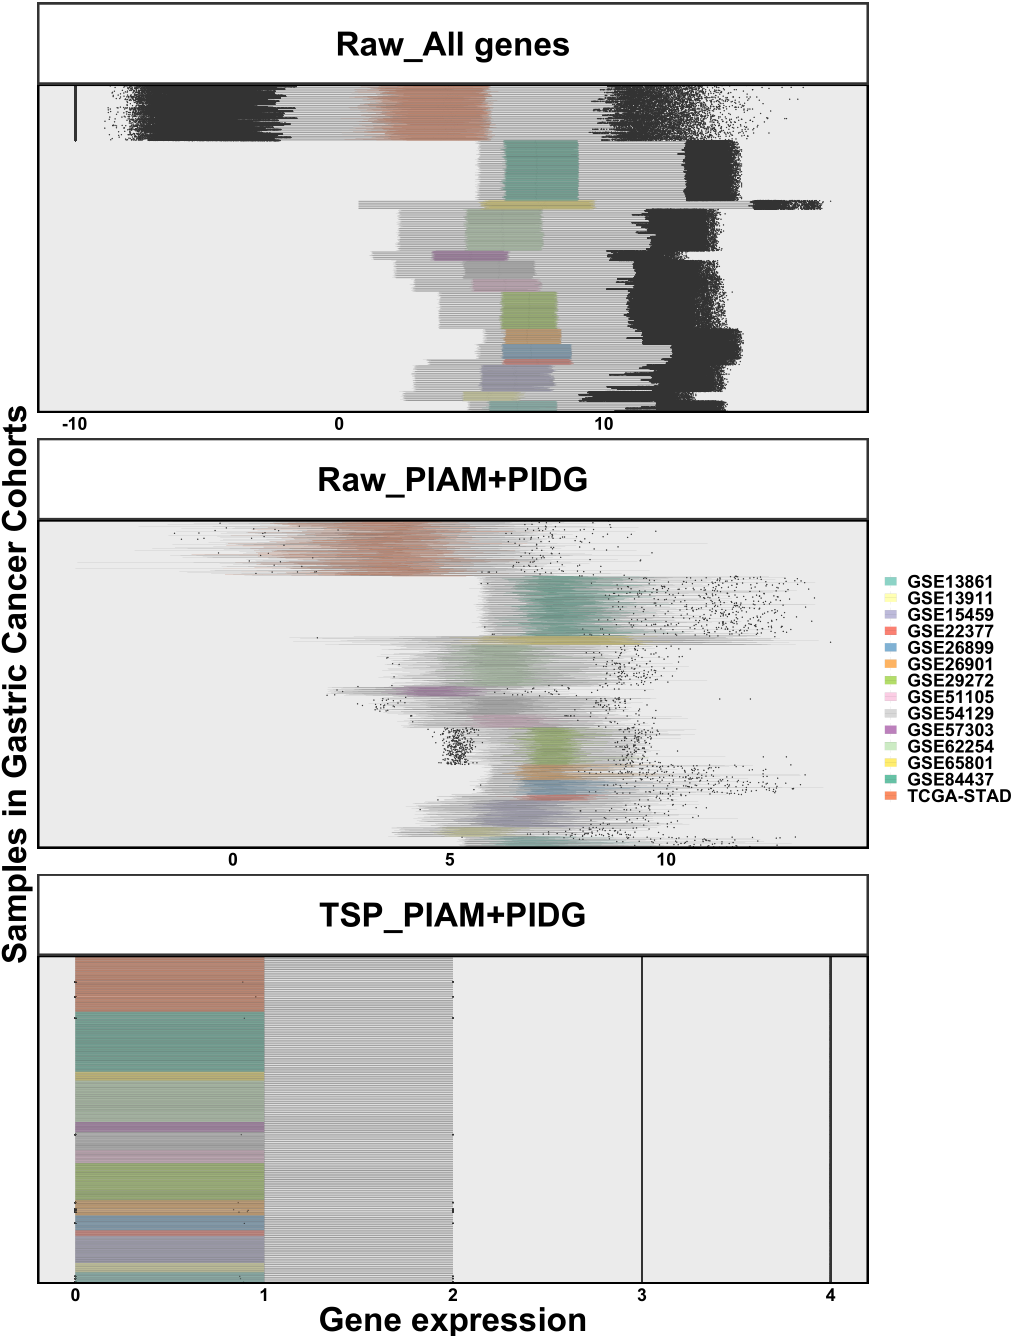
\includegraphics[width=0.9\linewidth]{./fig/bactch-effect-01} 

}

\caption{Batch effects across gastric cancer cohorts. All gene pairs were used because subtype vectors were not specified. Top: Raw expression of all genes across samples. Middle: Raw expression of PIAM and PIDG across samples. Bottom: TSP of PIAM and PIDG across samples.}\label{fig:be01}
\end{figure}

In order to confirmed the association between \textbf{gene counts} in modeling and batch effect control via \textbf{TSP} normalization, we selected random genes with counts ranging 4, 8, 20, 40, and 80 for TSP matrix establishment. As shown in Figure \ref{fig:be02}, \textbf{TSP} normalization works greatly in different gene counts for batch effect control compared with raw expression matrix.

\begin{figure}

{\centering 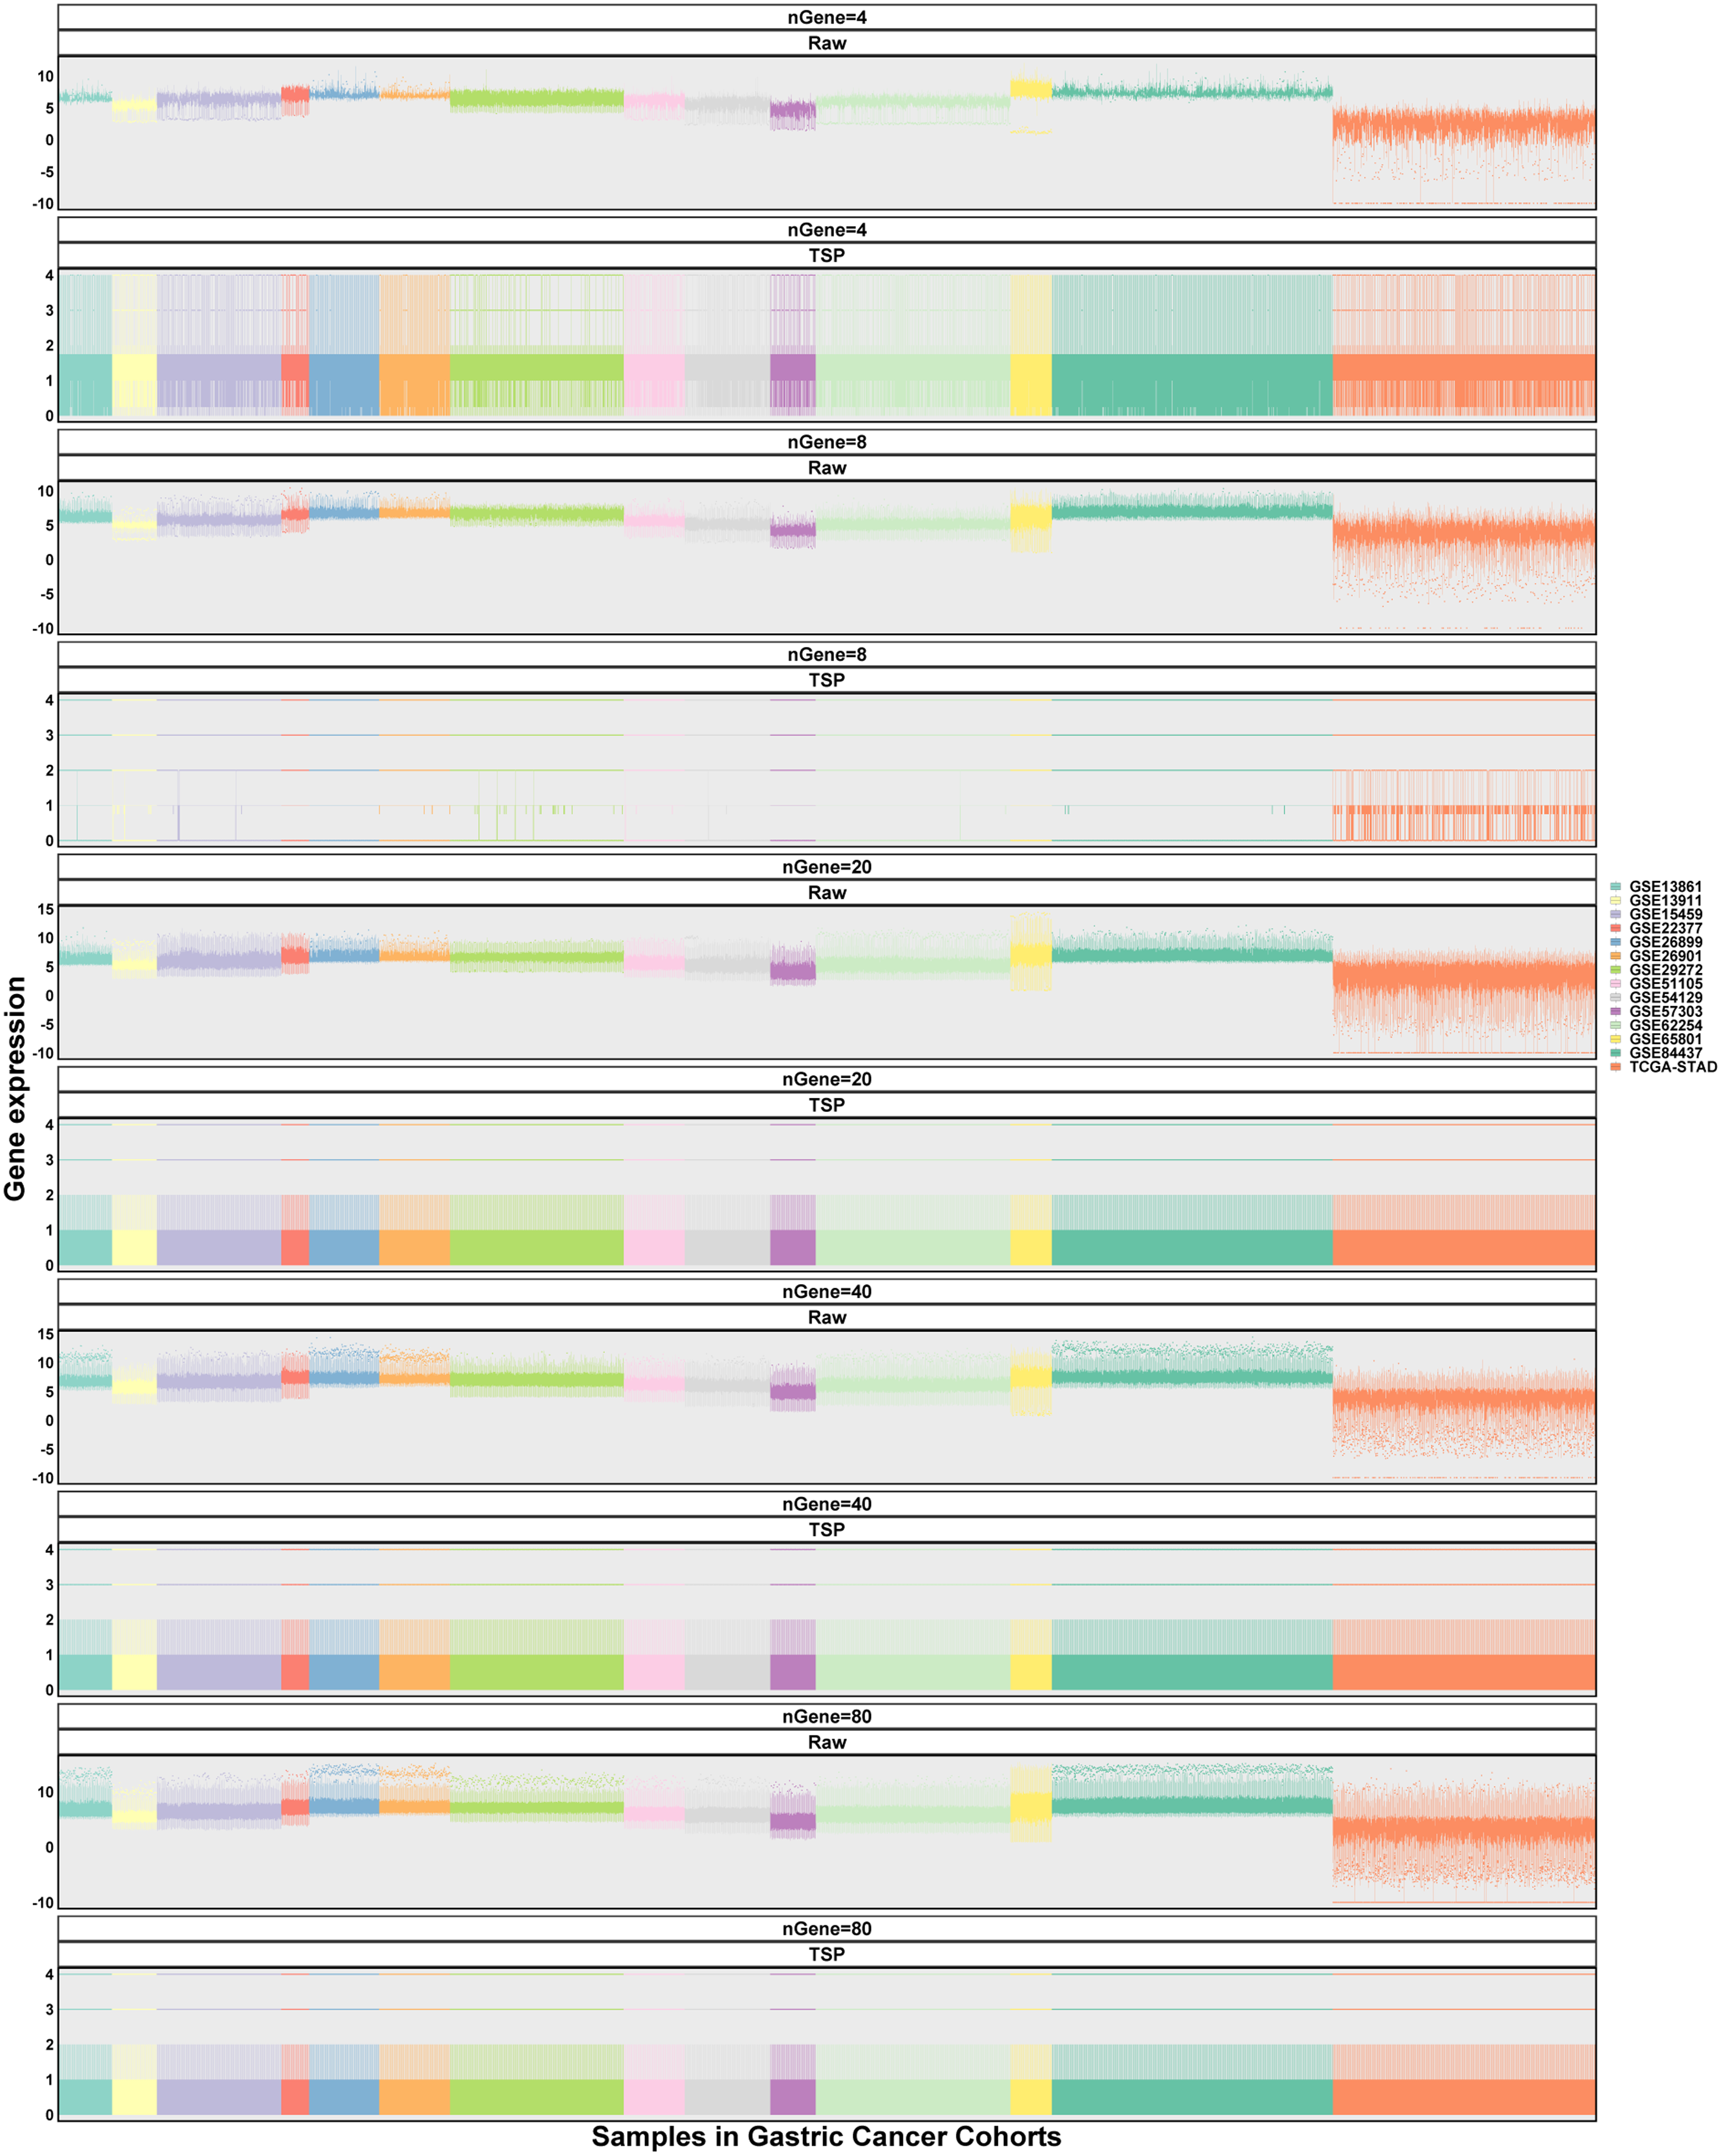
\includegraphics[width=0.9\linewidth]{./fig/bactch-effect-02} 

}

\caption{Batch effects of random genes across gastric cancer cohorts.  All gene pairs were used because subtype vectors were not specified. Gene counts 4, 8, 20, 40, and 80 were detected. Data of set difference were not available because only one gene set were applied.}\label{fig:be02}
\end{figure}

\hypertarget{hyperparameters}{%
\section{Hyperparameters}\label{hyperparameters}}

\hypertarget{quick-start}{%
\chapter{Quick start}\label{quick-start}}

\hypertarget{about}{%
\section{About}\label{about}}

\begin{itemize}
\tightlist
\item
  Although with bright prospects in Pan-disease analysis, \href{https://github.com/huangwb8/GSClassifier}{GSClassifier} was primarily developed for clinic-friendly immune subtypes of gastric cancer (GC). Currently, only \passthrough{\lstinline!PAD!} subtypes and \passthrough{\lstinline!PADi!} for GC were supported. We would try to support more cancer types in the future as possible. More details in \href{https://github.com/huangwb8/GSClassifier/wiki/Plans-in-the-future}{Plans in the future} section.
\item
  Gibbs' \passthrough{\lstinline!PanCancer immune subtypes!} based on five gene signatures (485 genes) could also be called in \passthrough{\lstinline!GSClassifier!}, with a pre-trained model from the \href{https://github.com/CRI-iAtlas/ImmuneSubtypeClassifier}{ImmuneSubtypeClassifier} package. If you use their jobs, please cite: \href{https://github.com/huangwb8/GSClassifier/wiki/Introduction\#Reference}{references}.
\item
  Particularly, all normal tissues should be eliminated before subtypes calling for cancer research.
\end{itemize}

\hypertarget{data}{%
\section{Data}\label{data}}

To lower the learning cost of \passthrough{\lstinline!GSClassifier!}, we provides some test data:

\begin{lstlisting}[language=R]
library(GSClassifier)
# 载入需要的程辑包:luckyBase
testData <- readRDS(system.file("extdata", "testData.rds", package = "GSClassifier"))
\end{lstlisting}

Explore the \passthrough{\lstinline!testData!}:

\begin{lstlisting}[language=R]
names(testData)
# [1] "Kim2018_3"              "PanSTAD_phenotype_part" "PanSTAD_expr_part"
\end{lstlisting}

\hypertarget{pad}{%
\section{PAD}\label{pad}}

\hypertarget{preparation-of-the-test-data}{%
\subsection{Preparation of the test data}\label{preparation-of-the-test-data}}

load phenotype data:

\begin{lstlisting}[language=R]
design <- testData$PanSTAD_phenotype_part
table(design$Dataset)
# 
#  GSE13861  GSE13911  GSE15459  GSE22377  GSE26899  GSE26901  GSE29272  GSE51105 
#        65        39       192        43        96       108       134        94 
#  GSE54129  GSE57303  GSE62254  GSE65801  GSE84437 TCGA-STAD 
#       111        70       300        32       433       372
\end{lstlisting}

load target sample IDs in \passthrough{\lstinline!GSE54129!} cohort:

\begin{lstlisting}[language=R]
target_ID <- design$ID[design$Dataset %in% 'GSE54129']
expr <- testData$PanSTAD_expr_part[,target_ID]
head(expr[,1:10])
#                 GSM1308413 GSM1308414 GSM1308415 GSM1308416 GSM1308417
# ENSG00000122122   7.888349   7.623663   6.873493   6.961102   7.150572
# ENSG00000117091   7.051760   6.217445   5.651839   5.830996   5.908532
# ENSG00000163219   6.056472   5.681844   5.411533   5.652684   5.555147
# ENSG00000136167   9.322191   8.765794   8.502315   8.838166   8.845952
# ENSG00000005844   7.119594   6.023631   5.400999   6.172863   6.059838
# ENSG00000123338   7.204051   6.925328   6.259809   6.610681   6.595882
#                 GSM1308418 GSM1308419 GSM1308420 GSM1308421 GSM1308422
# ENSG00000122122   7.871423   6.953329   8.334037   6.764335   6.522554
# ENSG00000117091   6.526917   5.646446   6.617520   5.637693   5.742848
# ENSG00000163219   5.962885   5.361763   5.975842   5.330428   5.172705
# ENSG00000136167   9.366074   8.675718   9.118517   8.614068   8.114096
# ENSG00000005844   6.523530   6.129181   7.331588   5.547059   5.867118
# ENSG00000123338   6.699790   6.935390   7.050288   6.536710   6.200269
\end{lstlisting}

\hypertarget{unsupervised-clustering}{%
\subsection{Unsupervised clustering}\label{unsupervised-clustering}}

\begin{lstlisting}[language=R]
res_pad <- PAD(
  expr = expr,
  cluster.method = "ward.D2",
  extra.annot = NULL,
  plot.title = 'PAD test',
  subtype = "PAD.train_20220916",
  verbose = T
)
\end{lstlisting}

\begin{center}\includegraphics[width=0.6\linewidth]{Quick-start_files/figure-latex/unnamed-chunk-5-1} \end{center}

\begin{lstlisting}
# Use default PIAM... 
# Use default PIDG... 
# Gene match: 100%. 
# Done!
\end{lstlisting}

\hypertarget{of-note}{%
\subsection{Of note}\label{of-note}}

\begin{itemize}
\item
  It's strongly recommanded that the gene type of \passthrough{\lstinline!expr!} should be alway the same, such as ENSEMBL genes (ENSG00000111640 for GAPDH, for examples).
\item
  \passthrough{\lstinline!PAD!} function is only for datasets with lots of samples for its classification depends on population-based unsupervised clusting. \passthrough{\lstinline!PAD!} is population-dependent and non-personalized.
\item
  Beta characteristics: You could try random forest classification based on the \passthrough{\lstinline!randomForest!} package or methods in \passthrough{\lstinline!stats::hclust!}.
\end{itemize}

\hypertarget{padi}{%
\section{PADi}\label{padi}}

\begin{itemize}
\item
  In \passthrough{\lstinline!GSClassifier!}, \passthrough{\lstinline!PADi!} is a pre-trained out-of-the-box model for GC personalized PAD subtypes calling.
\item
  During the sutype calling, the gene rank relations based on individuals instead of the relative values across samples would be used. Thus, \textbf{you don't have to do batch normalization} even though the data (the \passthrough{\lstinline!X!} input) come from multiple cohorts or platform.
\item
  More limitations were discussed in our paper that you had better know.
\end{itemize}

In this section, we would showed how to use \passthrough{\lstinline!PADi!} series: \passthrough{\lstinline!PADi!}, \passthrough{\lstinline!callEnsemble!}, and \passthrough{\lstinline!parCallEnsemble!} functions.

\hypertarget{preparation-of-the-test-data-1}{%
\subsection{Preparation of the test data}\label{preparation-of-the-test-data-1}}

\begin{lstlisting}[language=R]

 X <- testData$Kim2018_3
 head(X)
#                   PB-16-002   PB-16-003   PB-16-004
# ENSG00000121410  0.07075272 -2.08976724 -1.43569557
# ENSG00000148584 -1.49631022 -0.23917056  0.94827471
# ENSG00000175899 -0.77315329  0.52163146  0.91264015
# ENSG00000166535 -0.28860715 -0.45964255 -0.38401295
# ENSG00000256069 -0.25034243  0.06863867  0.14429081
# ENSG00000184389  0.08215945 -0.05966481  0.04937924
\end{lstlisting}

\hypertarget{use-a-specific-function-called-padi}{%
\subsection{\texorpdfstring{Use a specific function called \texttt{PADi}}{Use a specific function called PADi}}\label{use-a-specific-function-called-padi}}

Very simple, just:

\begin{lstlisting}[language=R]
res_padi <- PADi(X = X, verbose = F)
\end{lstlisting}

Check the result:

\begin{lstlisting}[language=R]
head(res_padi)
#   SampleIDs BestCall BestCall_Max           1          2          3         4
# 1 PB-16-002        4            4 0.023372779 0.02631794 0.04864784 0.3336484
# 2 PB-16-003        4            4 0.007271698 0.08650742 0.01974812 0.9530730
# 3 PB-16-004        4            4 0.011559768 0.02922151 0.09018894 0.8649045
\end{lstlisting}

Actually, \passthrough{\lstinline!PADi!} is exactly based on a general function called \passthrough{\lstinline!callEnsemble!}.

\hypertarget{use-the-callensemble-function}{%
\subsection{\texorpdfstring{Use the \texttt{callEnsemble} function}{Use the callEnsemble function}}\label{use-the-callensemble-function}}

Also simple, just:

\begin{lstlisting}[language=R]
res_padi <- callEnsemble(
    X = X,
    ens = NULL,
    geneAnnotation = NULL,
    geneSet = NULL,
    scaller = NULL,
    geneid = "ensembl",
    subtype = "PAD.train_20220916",
    verbose = F
  )
\end{lstlisting}

Check the result:

\begin{lstlisting}[language=R]
head(res_padi)
#   SampleIDs BestCall BestCall_Max          1          2          3         4
# 1 PB-16-002        4            4 0.01338872 0.01624520 0.03965218 0.8052567
# 2 PB-16-003        4            4 0.04709511 0.08833681 0.03879361 0.6244038
# 3 PB-16-004        4            4 0.01389035 0.03638009 0.05852707 0.6980438
\end{lstlisting}

\hypertarget{parallel-strategy-for-padi}{%
\subsection{Parallel strategy for PADi}\label{parallel-strategy-for-padi}}

\begin{itemize}
\item
  Sometimes, the number of patients for subtype callings could be huge (hundreds or even tens of thousands). Thus, the parallel computing (Windows or Linux pass; not tested in Mac or other OS) was also developed in the current version of \passthrough{\lstinline!GSClassifier!} package.
\item
  The parameter \passthrough{\lstinline!numCores!} was used to control the No.~of CPU for computing (which depends on your CPU capacity).
\end{itemize}

\begin{lstlisting}
# No run for the tiny test data. With errors.

# Method 1:
res_padi <- PADi(X = X, verbose = F, numCores = 4)

# Method 2: 
res_padi <- parCallEnsemble(
  X = X,
  ens = NULL,
  geneAnnotation = NULL,
  geneSet = NULL,
  scaller = NULL,
  geneids = 'ensembl',
  subtype = 'PAD.train_20220916',
  verbose = T,
  numCores = 4)
\end{lstlisting}

\hypertarget{single-sample-subtype-calling}{%
\subsection{Single sample subtype calling}\label{single-sample-subtype-calling}}

In clinical practice, the single sample subtype calling might be one of the most common scenarios and is also supported by functions of \passthrough{\lstinline!PADi!} series.

Supposed that there is a GC patient, its information should be:

\begin{lstlisting}[language=R]
X_ind <- X[,1]; names(X_ind) <- rownames(X)
head(X_ind)
# ENSG00000121410 ENSG00000148584 ENSG00000175899 ENSG00000166535 ENSG00000256069 
#      0.07075272     -1.49631022     -0.77315329     -0.28860715     -0.25034243 
# ENSG00000184389 
#      0.08215945
\end{lstlisting}

Or it can also be another format:

\begin{lstlisting}[language=R]
X_ind <- as.matrix(X[,1]); rownames(X_ind) <- rownames(X)
head(X_ind)
#                        [,1]
# ENSG00000121410  0.07075272
# ENSG00000148584 -1.49631022
# ENSG00000175899 -0.77315329
# ENSG00000166535 -0.28860715
# ENSG00000256069 -0.25034243
# ENSG00000184389  0.08215945
\end{lstlisting}

Similar to multiples sample calling, just:

check the result:

\begin{lstlisting}[language=R]
head(res_padi)
#   SampleIDs BestCall BestCall_Max          1          2          3         4
# 1    target        4            4 0.02337278 0.02631794 0.04864784 0.3336484
\end{lstlisting}

Similarly, there is alternative choice:

\begin{lstlisting}[language=R]
res_padi <- callEnsemble(
    X = X_ind,
    ens = NULL,
    geneAnnotation = NULL,
    geneSet = NULL,
    scaller = NULL,
    geneid = "ensembl",
    subtype = "PAD.train_20220916",
    verbose = F
  )
\end{lstlisting}

Check the result:

\begin{lstlisting}[language=R]
head(res_padi)
#   SampleIDs BestCall BestCall_Max          1         2          3         4
# 1    target        4            4 0.01338872 0.0162452 0.03965218 0.8052567
\end{lstlisting}

\hypertarget{of-note-1}{%
\subsection{Of note}\label{of-note-1}}

\begin{itemize}
\item
  In the results of \passthrough{\lstinline!PADi!}, two types of subtypes (\passthrough{\lstinline!BestCall!} and \passthrough{\lstinline!BestCall\_Max!}) were integrated. \passthrough{\lstinline!BestCall!} was predicted based on a xgboost-trained model based on prior knowlege of \passthrough{\lstinline!PAD!} subtypes and the possibility matrix (columns 4 to 7 of four-subtype calling, for example), while \passthrough{\lstinline!BestCall\_Max!} was predicted via maximum strategy. You should use THE SAME ONE in a specific practice no matter which one you use.
\item
  \passthrough{\lstinline!PADi!} is individual-dependent and personalized, which means that the result of subtype calling would not be influenced by the data of others.
\end{itemize}

\hypertarget{use-external-models-from-luckymodel-package}{%
\section{Use external models from luckyModel package}\label{use-external-models-from-luckymodel-package}}

In the future, there might be lots of models available as a resource of \passthrough{\lstinline!GSClassifier!}, such as \href{https://github.com/huangwb8/luckyModel}{luckyModel}. Here we show how \passthrough{\lstinline!luckyModel!} support \passthrough{\lstinline!GSClassifier!}.

First, intall and load \passthrough{\lstinline!luckyModel!}:

\begin{lstlisting}[language=R]
# Install luckyModel
if (!requireNamespace("luckyModel", quietly = TRUE))
    devtools::install_github("huangwb8/luckyModel")
library(luckyModel)
\end{lstlisting}

Check projects supported in current \passthrough{\lstinline!luckyModel!}:

\begin{lstlisting}[language=R]
list_project()
# [1] "GSClassifier"
\end{lstlisting}

Check available models in the project:

\begin{lstlisting}[language=R]
list_model(project='GSClassifier')
# Available models in GSClassifier:
#   *Gibbs_PanCancerImmuneSubtype_v20190731
#   *HWB_PAD_v20200110
\end{lstlisting}

Here, \passthrough{\lstinline!HWB\_PAD\_v20200110!} is a standard name of \passthrough{\lstinline!PADi!}. They are exactly the same.

Taking \passthrough{\lstinline!PADi!} as an example, we here show how to use an external model from \passthrough{\lstinline!luckyModel!}. First, load a model:

\begin{lstlisting}[language=R]
model <- lucky_model(project = 'GSClassifier',
                     developer='HWB',
                     model = 'PAD',
                     version = 'v20200110')
\end{lstlisting}

Then, check the gene id type:

\begin{lstlisting}[language=R]
model$geneSet
# $PIAM
#  [1] "ENSG00000122122" "ENSG00000117091" "ENSG00000163219" "ENSG00000136167"
#  [5] "ENSG00000005844" "ENSG00000123338" "ENSG00000102879" "ENSG00000010671"
#  [9] "ENSG00000185862" "ENSG00000104814" "ENSG00000134516" "ENSG00000100055"
# [13] "ENSG00000082074" "ENSG00000113263" "ENSG00000153283" "ENSG00000198821"
# [17] "ENSG00000185811" "ENSG00000117090" "ENSG00000171608"
# 
# $PIDG
#  [1] "ENSG00000116667" "ENSG00000107771" "ENSG00000196782" "ENSG00000271447"
#  [5] "ENSG00000173517" "ENSG00000134686" "ENSG00000100614" "ENSG00000134247"
#  [9] "ENSG00000109686" "ENSG00000197321" "ENSG00000179981" "ENSG00000187189"
# [13] "ENSG00000140836"
\end{lstlisting}

The model should use \passthrough{\lstinline!ensembl!} as the value of \passthrough{\lstinline!geneid!} parameter in \passthrough{\lstinline!callEnsemble!} series.

Next, you can use the model like:

\begin{lstlisting}[language=R]
res_padi <- callEnsemble(
  X = X,
  ens = model$ens$Model,
  geneAnnotation = model$geneAnnotation,
  geneSet = model$geneSet,
  scaller = model$scaller$Model,
  geneid = "ensembl",
  subtype = NULL,
  verbose = F
)
\end{lstlisting}

Or just:

\begin{lstlisting}[language=R]
res_padi <- callEnsemble(
  X,
  ens = NULL,
  geneAnnotation = NULL,
  geneSet = NULL,
  scaller = NULL,
  geneid = "ensembl",
  subtype = model, 
  verbose = F
)
\end{lstlisting}

They are exactly the same.

Finally, check the result:

\begin{lstlisting}[language=R]
head(res_padi)
#   SampleIDs BestCall BestCall_Max           1          2          3         4
# 1 PB-16-002        4            4 0.023372779 0.02631794 0.04864784 0.3336484
# 2 PB-16-003        4            4 0.007271698 0.08650742 0.01974812 0.9530730
# 3 PB-16-004        4            4 0.011559768 0.02922151 0.09018894 0.8649045
\end{lstlisting}

\hypertarget{pancancer-immune-subtypes}{%
\section{PanCancer immune subtypes}\label{pancancer-immune-subtypes}}

\passthrough{\lstinline!GSClassifier!} could also call the \passthrough{\lstinline!PanCancer immune subtypes!} of Gibbs'.

First, see data available in current \passthrough{\lstinline!GSClassifier!}:

\begin{lstlisting}[language=R]
GSClassifier_Data()
# Available data:
# Usage example:
#   ImmuneSubtype.rds 
#   PAD.train_20200110.rds 
#   PAD.train_20220916.rds 
#   PAD <- readRDS(system.file("extdata", "PAD.train_20200110.rds", package = "GSClassifier")) 
#   ImmuneSubtype <- readRDS(system.file("extdata", "ImmuneSubtype.rds", package = "GSClassifier"))
\end{lstlisting}

Let's use our test data to do this:

\begin{lstlisting}[language=R]

X <- testData$Kim2018_3
symbol <- convert(rownames(X))
rownames(X) <- symbol
X <- X[!is.na(symbol),]
dim(X)
# [1] 19118     3
\end{lstlisting}

Have a check

\begin{lstlisting}[language=R]
head(X)
#                 PB-16-002   PB-16-003   PB-16-004
# A1BG           0.07075272 -2.08976724 -1.43569557
# A1CF          -1.49631022 -0.23917056  0.94827471
# A2M           -0.77315329  0.52163146  0.91264015
# A2ML1         -0.28860715 -0.45964255 -0.38401295
# RP11-118B22.6 -0.25034243  0.06863867  0.14429081
# A3GALT2        0.08215945 -0.05966481  0.04937924
\end{lstlisting}

PanCan Immune Subtype callings:

\begin{lstlisting}[language=R]
res_pis <- callEnsemble(
    X = X,
    ens = NULL,
    geneAnnotation = NULL,
    geneSet = NULL,
    scaller = NULL,
    geneid = "symbol",
    subtype = "ImmuneSubtype",
    verbose = F
  )
\end{lstlisting}

Check the result:

\begin{lstlisting}[language=R]
head(res_pis)
#   SampleIDs BestCall BestCall_Max            1           2            3
# 1 PB-16-002        2            2 8.928682e-04 0.561300665 9.943818e-06
# 2 PB-16-003        4            4 4.040183e-07 0.018167170 1.258724e-04
# 3 PB-16-004        3            3 6.196300e-06 0.001126488 2.408393e-01
#             4           5           6
# 1 0.279268414 0.010949500 0.003348467
# 2 0.499039710 0.002884648 0.001938546
# 3 0.000298221 0.007653435 0.005676751
\end{lstlisting}

Also, you can try to use \passthrough{\lstinline!luckyModel!}:

\begin{lstlisting}[language=R]
pci <- lucky_model(
  project = "GSClassifier",
  model = "PanCancerImmuneSubtype",
  developer = "Gibbs",
  version = "v20190731"
)
\end{lstlisting}

PanCan Immune Subtype callings:

\begin{lstlisting}[language=R]
res_pis <- callEnsemble(
    X = X,
    ens = NULL,
    geneAnnotation = NULL,
    geneSet = NULL,
    scaller = NULL,
    geneid = "symbol",
    subtype = pci,
    verbose = F
  )
\end{lstlisting}

Finally, we take a look at the \passthrough{\lstinline!PanCancer immune subtypes!} model:

\begin{lstlisting}[language=R]
ImmuneSubtype <- readRDS(system.file("extdata", "ImmuneSubtype.rds", package = "GSClassifier"))
names(ImmuneSubtype)
# [1] "ens"            "scaller"        "geneAnnotation" "geneSet"
\end{lstlisting}

Its gene annotation:

\begin{lstlisting}[language=R]
head(ImmuneSubtype$geneAnnotation)
#      SYMBOL ENTREZID         ENSEMBL
# 235  ACTL6A       86 ENSG00000136518
# 294   ADAM9     8754 ENSG00000168615
# 305 ADAMTS1     9510 ENSG00000154734
# 322    ADAR      103 ENSG00000160710
# 340   ADCY7      113 ENSG00000121281
# 479   AIMP2     7965 ENSG00000106305
\end{lstlisting}

Its gene sets:

\begin{lstlisting}[language=R]
ImmuneSubtype$geneSet
# $LIexpression_score
#  [1] "CCL5"  "CD19"  "CD37"  "CD3D"  "CD3E"  "CD3G"  "CD3Z"  "CD79A" "CD79B"
# [10] "CD8A"  "CD8B1" "IGHG3" "IGJ"   "IGLC1" "CD14"  "LCK"   "LTB"   "MS4A1"
# 
# $CSF1_response
#   [1] "CORO1A"   "MNDA"     "CCRL2"    "SLC7A7"   "HLA-DMA"  "FYB"     
#   [7] "RNASE6"   "TLR2"     "CTSC"     "LILRB4"   "PSCDBP"   "CTSS"    
#  [13] "RASSF4"   "MSN"      "CYBB"     "LAPTM5"   "DOCK2"    "FCGR1A"  
#  [19] "EVI2B"    "ADCY7"    "CD48"     "ARHGAP15" "ARRB2"    "SYK"     
#  [25] "BTK"      "TNFAIP3"  "FCGR2A"   "VSIG4"    "FPRL2"    "IL10RA"  
#  [31] "IFI16"    "ITGB2"    "IL7R"     "TBXAS1"   "FMNL1"    "FLI1"    
#  [37] "RASSF2"   "LYZ"      "CD163"    "CD97"     "CCL2"     "FCGR2B"  
#  [43] "MERTK"    "CD84"     "CD53"     "CD86"     "HMHA1"    "CTSL"    
#  [49] "EVI2A"    "TNFRSF1B" "CXCR4"    "LCP1"     "SAMHD1"   "CPVL"    
#  [55] "HLA-DRB1" "C13orf18" "GIMAP4"   "SAMSN1"   "PLCG2"    "OSBPL3"  
#  [61] "CD8A"     "RUNX3"    "FCGR3A"   "AMPD3"    "MYO1F"    "CECR1"   
#  [67] "LYN"      "MPP1"     "LRMP"     "FGL2"     "NCKAP1L"  "HCLS1"   
#  [73] "SELL"     "CASP1"    "SELPLG"   "CD33"     "GPNMB"    "NCF2"    
#  [79] "FNBP1"    "IL18"     "B2M"      "SP140"    "FCER1G"   "LCP2"    
#  [85] "LY86"     "LAIR1"    "IFI30"    "TNFSF13B" "LST1"     "FGR"     
#  [91] "NPL"      "PLEK"     "CCL5"     "PTPRC"    "GNPTAB"   "SLC1A3"  
#  [97] "HCK"      "NPC2"     "C3AR1"    "PIK3CG"   "DAPK1"    "ALOX5AP" 
# [103] "CSF1R"    "CUGBP2"   "APOE"     "APOC1"    "CD52"     "LHFPL2"  
# [109] "C1orf54"  "IKZF1"    "SH2B3"    "WIPF1"   
# 
# $Module3_IFN_score
#  [1] "IFI44"  "IFI44L" "DDX58"  "IFI6"   "IFI27"  "IFIT2"  "IFIT1"  "IFIT3" 
#  [9] "CXCL10" "MX1"    "OAS1"   "OAS2"   "OAS3"   "HERC5"  "SAMD9"  "HERC6" 
# [17] "DDX60"  "RTP4"   "IFIH1"  "STAT1"  "TAP1"   "OASL"   "RSAD2"  "ISG15" 
# 
# $TGFB_score_21050467
#  [1] "MMP3"     "MARCKSL1" "IGF2R"    "LAMB1"    "SPARC"    "FN1"     
#  [7] "ITGA4"    "SMO"      "MMP19"    "ITGB8"    "ITGA5"    "NID1"    
# [13] "TIMP1"    "SEMA3F"   "RHOQ"     "CTNNB1"   "MMP2"     "SERPINE1"
# [19] "EPHB2"    "COL16A1"  "EPHA2"    "TNC"      "JUP"      "ITGA3"   
# [25] "TCF7L2"   "COL3A1"   "CDH6"     "WNT2B"    "ADAM9"    "DSP"     
# [31] "HSPG2"    "ARHGAP1"  "ITGB5"    "IGFBP5"   "ARHGDIA"  "LRP1"    
# [37] "IGFBP2"   "CTNNA1"   "LRRC17"   "MMP14"    "NEO1"     "EFNA5"   
# [43] "ITGB3"    "EPHB3"    "CD44"     "IGFBP4"   "TNFRSF1A" "RAC1"    
# [49] "PXN"      "PLAT"     "COL8A1"   "WNT8B"    "IGFBP3"   "RHOA"    
# [55] "EPHB4"    "MMP1"     "PAK1"     "MTA1"     "THBS2"    "CSPG2"   
# [61] "MMP17"    "CD59"     "DVL3"     "RHOB"     "COL6A3"   "NOTCH2"  
# [67] "BSG"      "MMP11"    "COL1A2"   "ZYX"      "RND3"     "THBS1"   
# [73] "RHOG"     "ICAM1"    "LAMA4"    "DVL1"     "PAK2"     "ITGB2"   
# [79] "COL6A1"   "FGD1"    
# 
# $CHANG_CORE_SERUM_RESPONSE_UP
#   [1] "CEP78"     "LSM3"      "LRRC40"    "STK17A"    "RPN1"      "JUNB"     
#   [7] "NUP85"     "FLNC"      "HMGN2"     "RPP40"     "UQCR10"    "AIMP2"    
#  [13] "CHEK1"     "VTA1"      "EXOSC8"    "CENPO"     "PNO1"      "SLC16A1"  
#  [19] "WDR77"     "UBE2J1"    "NOP16"     "NUDT1"     "SMC2"      "SLC25A5"  
#  [25] "NUPL1"     "DLEU2"     "PDAP1"     "CCBL2"     "COX17"     "BCCIP"    
#  [31] "PLG"       "RGS8"      "SNRPC"     "PLK4"      "NUTF2"     "LSM4"     
#  [37] "SMS"       "EBNA1BP2"  "C13orf27"  "VDAC1"     "PSMD14"    "MYCBP"    
#  [43] "SMURF2"    "GNG11"     "F3"        "IL7R"      "BRIP1"     "HNRNPA2B1"
#  [49] "DCK"       "ALKBH7"    "HN1L"      "MSN"       "TPM1"      "HYLS1"    
#  [55] "HAUS1"     "NUP93"     "SNRPE"     "ITGA6"     "CENPN"     "C11orf24" 
#  [61] "GGH"       "PFKP"      "FARSA"     "EIF2AK1"   "CENPW"     "TUBA4A"   
#  [67] "TRA2B"     "UMPS"      "MRTO4"     "NUDT15"    "PGM2"      "DBNDD1"   
#  [73] "SNRPB"     "MNAT1"     "NUP35"     "TCEB1"     "HSPB11"    "C19orf48" 
#  [79] "ID3"       "IPO4"      "FARSB"     "EIF4G1"    "SKA1"      "MFSD11"   
#  [85] "PLAUR"     "MARVELD2"  "MCM3"      "DHFR"      "RNF41"     "ID2"      
#  [91] "H2AFZ"     "CDK2"      "NCLN"      "ZWILCH"    "DYNLT1"    "C16orf61" 
#  [97] "SLC25A40"  "RHOC"      "CCT5"      "PDIA4"     "SNRPA"     "RBM14"    
# [103] "PDLIM7"    "PITPNC1"   "TPM3"      "CORO1C"    "ERLIN1"    "PAICS"    
# [109] "TPRKB"     "SKA2"      "MYBL1"     "SH3BP5L"   "BRCA2"     "SAR1A"    
# [115] "POLR3K"    "MRPS28"    "NUP107"    "TUBG1"     "PNN"       "FAM167A"  
# [121] "RFC3"      "MYL6"      "MCM7"      "MAGOHB"    "FAM89B"    "TOMM40"   
# [127] "CDCA4"     "MT3"       "MTHFD1"    "PSMD12"    "MYBL2"     "CKLF"     
# [133] "NRIP3"     "EZR"       "C12orf24"  "GPLD1"     "SRM"       "RAB3B"    
# [139] "NLN"       "MT1F"      "TNFRSF12A" "TPI1"      "HAS2"      "APOO"     
# [145] "FBXO41"    "MRPL37"    "GSTCD"     "SDC1"      "WDR54"     "RNF138"   
# [151] "APITD1"    "RMND5B"    "ENO1"      "MAP3K8"    "TMEM130"   "SNX17"    
# [157] "KRR1"      "TAGLN"     "PA2G4"     "RUVBL1"    "SNRPD1"    "LOXL2"    
# [163] "POLE2"     "MAPRE1"    "IMP4"      "EMP2"      "PSMD2"     "MET"      
# [169] "IFRD2"     "LMNB2"     "PLOD2"     "NCEH1"     "NME1"      "STRA13"   
# [175] "ACTL6A"    "DLEU1"     "SNRPA1"    "CBX1"      "LYAR"      "PTPLB"    
# [181] "PFN1"      "CENPJ"     "COTL1"     "SPRYD7"    "USPL1"     "MRPL12"   
# [187] "ADAMTS1"   "GLRX3"     "WSB2"      "MRPS16"    "DCLRE1B"   "MKKS"     
# [193] "C3orf26"   "CPEB4"     "SPAG17"    "MLF1IP"    "UAP1"      "COQ2"     
# [199] "WDHD1"     "DCBLD2"    "KIAA0090"  "SAR1B"     "PSMA7"     "PSMC3"    
# [205] "COPS6"     "DUT"       "PPIH"      "PHF19"     "TPM2"      "MCTS1"    
# [211] "EIF4EBP1"  "HNRNPR"
\end{lstlisting}

Enjoy \passthrough{\lstinline!GSClassifier!}!

\hypertarget{model-establishment-via-gsclassifier}{%
\chapter{Model establishment via GSClassifier}\label{model-establishment-via-gsclassifier}}

\hypertarget{about-1}{%
\section{About}\label{about-1}}

Sometimes, researchers might have their own gene signatures and know how many subtypes they want to call before (based on some knowledges). Gratifyingly, comprehensive functions were also provided in \passthrough{\lstinline!GSClassifier!}. In this section, we would show how to build a \passthrough{\lstinline!GSClassifier!} model like \passthrough{\lstinline!PADi!}.

\hypertarget{data-preparation}{%
\section{Data preparation}\label{data-preparation}}

\begin{quote}
Note: The test data is only for the demonstration of the modeling
\end{quote}

Load packages:

Load data:

\begin{lstlisting}[language=R]
testData <- readRDS(system.file("extdata", "testData.rds", package = "GSClassifier"))
expr <- testData$PanSTAD_expr_part
design <- testData$PanSTAD_phenotype_part
\end{lstlisting}

Select training and testing cohorts across different platforms and \passthrough{\lstinline!PAD subtypes!} from \passthrough{\lstinline!PAD!} function:

\begin{lstlisting}[language=R]
modelInfo <- modelData(
    design,
    id.col = "ID",
    variable = c("platform", "PAD_subtype"),
    Prop = 0.7,
    seed = 145
  )
\end{lstlisting}

Check the result \passthrough{\lstinline!modelInfo!}:

\begin{lstlisting}[language=R]
names(modelInfo)

head(modelInfo$Data$Train)

head(modelInfo$Data$Valid)
# [1] "Repeat" "Data"  
#                    ID  Dataset PAD_subtype PIAM_subtype PIDG_subtype platform
# GSM1606509 GSM1606509 GSE65801       PAD-I         high         high GPL14550
# GSM1606517 GSM1606517 GSE65801       PAD-I         high         high GPL14550
# GSM1606503 GSM1606503 GSE65801       PAD-I         high         high GPL14550
# GSM1606525 GSM1606525 GSE65801       PAD-I         high         high GPL14550
# GSM1606511 GSM1606511 GSE65801       PAD-I         high         high GPL14550
# GSM1606527 GSM1606527 GSE65801       PAD-I         high         high GPL14550
#                    ID  Dataset PAD_subtype PIAM_subtype PIDG_subtype platform
# GSM2235558 GSM2235558 GSE84437       PAD-I         high         high  GPL6947
# GSM2235561 GSM2235561 GSE84437      PAD-II         high          low  GPL6947
# GSM2235562 GSM2235562 GSE84437      PAD-IV          low          low  GPL6947
# GSM2235563 GSM2235563 GSE84437      PAD-IV          low          low  GPL6947
# GSM2235564 GSM2235564 GSE84437      PAD-IV          low          low  GPL6947
# GSM2235567 GSM2235567 GSE84437      PAD-IV          low          low  GPL6947
\end{lstlisting}

Get training data \passthrough{\lstinline!Xs!} and \passthrough{\lstinline!Ys!}:

\begin{lstlisting}[language=R]
  # Training data
  Xs <- expr[,modelInfo$Data$Train$ID]
  y <- modelInfo$Data$Train
  y <- y[colnames(Xs),]
  Ys <- ifelse(y$PAD_subtype == 'PAD-I',1,ifelse(y$PAD_subtype == 'PAD-II',2,ifelse(y$PAD_subtype == 'PAD-III',3,ifelse(y$PAD_subtype == 'PAD-IV',4,NA)))); table(Ys)/length(Ys)
# Ys
#         1         2         3         4 
# 0.1010169 0.2474576 0.1694915 0.4820339
\end{lstlisting}

Get the number of subtype:

\begin{lstlisting}[language=R]
# No. of subtypes
nSubtype <- length(unique(Ys))
print(nSubtype)
# [1] 4
\end{lstlisting}

Also, you can take a look at the validation data:

\begin{lstlisting}[language=R]
# Validating data
Xs_valid <- expr[,modelInfo$Data$Valid$ID]
y <- modelInfo$Data$Valid
y <- y[colnames(Xs_valid),]
Ys_valid <- ifelse(y$PAD_subtype == 'PAD-I',1,ifelse(y$PAD_subtype == 'PAD-II',2,ifelse(y$PAD_subtype == 'PAD-III',3,ifelse(y$PAD_subtype == 'PAD-IV',4,NA))))
table(Ys_valid)/length(Ys_valid)
# Ys_valid
#          1          2          3          4 
# 0.09609121 0.24592834 0.16612378 0.49185668
\end{lstlisting}

Note: When you convert your phenotype into numeric, \textbf{You CANNOT USE A ZERO VALUE}, which is not supported by the xGboost.

Other parameteres for modeling:

\begin{lstlisting}[language=R]

# Build 20 models
n=20 

# In every model, 70% samples in the training cohort would be selected. 
sampSize=0.7

# Seed for sampling
sampSeed = 2020
na.fill.seed = 2022

# A vector for approximate gene rank estimation
breakVec=c(0, 0.25, 0.5, 0.75, 1.0)
  
# Use 80% most variable gene & gene-pairs for modeling
ptail=0.8/2

# Automatical selection of parameters for xGboost
auto = F

if(!auto){
      
      # Self-defined params. Fast.
      params = list(max_depth = 10,
                    eta = 0.5,
                    nrounds = 100,
                    nthread = 10,
                    nfold=5)
      caret.seed = NULL
      
      # No. of CPU for parallel computing. The optimized value depends on your CPU and RAM
      numCores = 4
      
    } else {
      
      # caret::train strategy by GSClassifier:::cvFitOneModel2. Time consuming
      params = NULL
      caret.seed = 105
      
      # Self-defined. For this exmaple training grid, there are 2×1×1×3×2×1×2=24 grids. Make sure that you have a computer with a powerfull CPU.
      grid = expand.grid(
        nrounds = c(100, 200),
        colsample_bytree = 1,
        min_child_weight = 1,
        eta = c(0.01, 0.1, 0.3),
        gamma = c(0.5, 0.3),
        subsample = 0.7,
        max_depth = c(5,8)
      )
      
      # If you don't know how to set, just use the same number of your subtypes
      numCores = 4 
    }
\end{lstlisting}

Finaly, you have to provide your gene sets as a \passthrough{\lstinline!list!} object:

\begin{lstlisting}
geneSet = <Your gene sets>
\end{lstlisting}

Let's take \passthrough{\lstinline!PAD!} as an example:

\begin{lstlisting}[language=R]
PAD <- readRDS(system.file("extdata", "PAD.train_20220916.rds", package = "GSClassifier"))
geneSet <- PAD$geneSet
print(geneSet)
# $PIAM
#  [1] "ENSG00000122122" "ENSG00000117091" "ENSG00000163219" "ENSG00000136167"
#  [5] "ENSG00000005844" "ENSG00000123338" "ENSG00000102879" "ENSG00000010671"
#  [9] "ENSG00000185862" "ENSG00000104814" "ENSG00000134516" "ENSG00000100055"
# [13] "ENSG00000082074" "ENSG00000113263" "ENSG00000153283" "ENSG00000198821"
# [17] "ENSG00000185811" "ENSG00000117090" "ENSG00000171608"
# 
# $PIDG
#  [1] "ENSG00000116667" "ENSG00000107771" "ENSG00000196782" "ENSG00000271447"
#  [5] "ENSG00000173517" "ENSG00000134686" "ENSG00000100614" "ENSG00000134247"
#  [9] "ENSG00000109686" "ENSG00000197321" "ENSG00000179981" "ENSG00000187189"
# [13] "ENSG00000140836"
\end{lstlisting}

\hypertarget{fitting-models}{%
\section{Fitting models}\label{fitting-models}}

\hypertarget{gsclassifier-model-training}{%
\subsection{GSClassifier model training}\label{gsclassifier-model-training}}

Just fit the model like:

\begin{lstlisting}

if(!auto){
  
  # Self-defined
  
  system.time(
    res <- fitEnsembleModel(Xs,
                            Ys,
                            geneSet = geneSet,
                            na.fill.method = c('quantile','rpart',NULL)[1],
                            na.fill.seed = na.fill.seed,
                            n = n,
                            sampSize = sampSize,
                            sampSeed = sampSeed ,
                            breakVec = breakVec,
                            params = params,
                            ptail = ptail,
                            caret.grid = NULL,
                            caret.seed =  caret.seed,
                            verbose = verbose,
                            numCores = numCores)
  )
  
  # user   system  elapsed
  # 0.08s  0.18s   92.70s
  
} else {
  
  # caret::train-defined and time-consuming
  system.time(
    res <- fitEnsembleModel(Xs,
                            Ys,
                            geneSet = geneSet,
                            na.fill.method = c('quantile','rpart',NULL)[1],
                            na.fill.seed = na.fill.seed,
                            n = n,
                            sampSize = sampSize,
                            sampSeed = sampSeed ,
                            breakVec = breakVec,
                            params = NULL,  # This must be NULL
                            ptail = ptail,
                            caret.grid = grid,
                            caret.seed =  caret.seed,
                            verbose = verbose,
                            numCores = numCores)
  )
  
  # user   system   elapsed
  # 1.10s  2.60s    2311.55s
}

mymusic() # Remind me with a music when the process completed
\end{lstlisting}

You should save it for convenience:

\begin{lstlisting}
saveRDS(res,'<your path>/train_ens.rds')
\end{lstlisting}

Although a \passthrough{\lstinline!auto-parameter strategy!} was provided in\passthrough{\lstinline!GSClassifier!}, it's unknown for this method to improve your model performance to what extent. You can just try. It's not a prior recommendation. In generall, setting \passthrough{\lstinline!auto=F!} in this script could be more cost-effective. Empirically, the speed of \passthrough{\lstinline!caret::train!} depends on single-core performance of the CPU instead of the core number.

\hypertarget{scaller-for-the-best-call}{%
\subsection{Scaller for the best call}\label{scaller-for-the-best-call}}

Next, we model the \passthrough{\lstinline!scaller!} for the training cohort, which would be used for \passthrough{\lstinline!BestCall!} based on the \passthrough{\lstinline!probability matrix!} in \passthrough{\lstinline!callEnsemble!} series. Here, \passthrough{\lstinline!scaller=NULL!} would cause an \passthrough{\lstinline!NA!} value of \passthrough{\lstinline!BestCall!} col.~It's not a big deal, because the \passthrough{\lstinline!probability matrix!} is the information we need.

\begin{lstlisting}
# Time-consuming modeling
resTrain <- parCallEnsemble(X = Xs,
                            ens = res$Model,
                            geneAnnotation = res$geneAnnotation,
                            geneSet = geneSet,
                            scaller = NULL,
                            geneids = "ensembl",
                            subtype = NULL,
                            numCores = numCores)

# xgboost via best interation
library(xgboost)
dtrain <- xgb.DMatrix(as.matrix(resTrain[4:(3 + nSubtype)]), label = Ys-1)

cvRes <- xgb.cv(data = dtrain,
                nrounds=100,
                nthread=10,
                nfold=5,
                max_depth=5,
                eta=0.5,
                early_stopping_rounds=100,
                num_class = 4,
                objective = "multi:softmax")

# xgboost via best interation
bst <- xgboost(data = dtrain,
               max_depth=5,
               eta=0.5,
               nrounds = cvRes$best_iteration,
               nthread=10,
               num_class = 4,
               objective = "multi:softmax")
Ys_pred <- predict(bst, as.matrix(resTrain[4:7])) + 1
mean(Ys_pred == Ys) # Prediction rates

# Ensemble results
scaller.train <- list(
      Repeat = list(
        data = dtrain,
        max_depth=5,
        eta=0.5,
        nrounds = cvRes$best_iteration,
        nthread=10,
        num_class = 4,
        objective = "multi:softmax"
      ), 
      Model = bst
    )
\end{lstlisting}

\hypertarget{assemble-your-model}{%
\subsection{Assemble your model}\label{assemble-your-model}}

\begin{quote}
For more information of \passthrough{\lstinline!geneAnnotation!}, you could see \href{https://github.com/huangwb8/GSClassifier/wiki/Advanced-development\#Gene-Annotation}{Advanced development: Gene Annotation} section for assistance.
\end{quote}

Here we give an example:

\begin{lstlisting}
l.train <- list()

# bootstrap models based on the training cohort
l.train[['ens']] <- res 

# Scaller model
l.train[['scaller']] <- scaller.train 

# a data frame contarining gene annotation for IDs convertion
l.train[['geneAnnotation']] <- <Your gene annotation>

# Your gene sets
l.train[['geneSet']] <- geneSet
\end{lstlisting}

Finally, save it for downstream analysis

\begin{lstlisting}
saveRDS(l.train,'<Your path>/train.rds')
\end{lstlisting}

About model constributions, you can go \passthrough{\lstinline!Advanced development!} in \href{https://github.com/huangwb8/GSClassifier/wiki/Advanced-development}{here} or \href{http://htmlpreview.github.io/?https://raw.githubusercontent.com/wiki/huangwb8/GSClassifier/Advanced-development.html}{here} for more information.

\hypertarget{of-note-2}{%
\subsection{Of note}\label{of-note-2}}

You can take a look at the \passthrough{\lstinline!PAD.train\_20220916!} model (\passthrough{\lstinline!PADi!}). You have to make your model frame similar to the \passthrough{\lstinline!PAD.train\_20220916!} model.

\begin{lstlisting}[language=R]
l.train <- readRDS(system.file("extdata", "PAD.train_20220916.rds", package = "GSClassifier"))
names(l.train)
# [1] "ens"            "scaller"        "geneAnnotation" "geneSet"
\end{lstlisting}

The time of \passthrough{\lstinline!GSClassifier!} modeling depends on the number of individual models (controlled by \passthrough{\lstinline!n!})/called subtypes/gene signatures, automatic parameter selection, and your CPU capacity.

\hypertarget{calling-subtypes}{%
\section{Calling subtypes}\label{calling-subtypes}}

Supposed that you had got a \passthrough{\lstinline!GSClassifier!} model, next you want to use it for personalized subtype calling.

Just:

\begin{lstlisting}
# Load your model
l <- readRDS('<Your path>/train.rds')

# subtype calling
res_i = callEnsemble(
  X,
  ens = l$ens$Model,
  geneAnnotation = l$geneAnnotation,
  geneSet = l$geneSet,
  scaller = l$scaller$Model,
  geneid = <ID type of your training data>,
  subtype = NULL,
  verbose = T
)
\end{lstlisting}

The usage of \passthrough{\lstinline!parCallEnsemble!} (for huge amount of samples) is similar.

\hypertarget{suggestions-for-gsclassifier-model-developers}{%
\chapter{Suggestions for GSClassifier model developers}\label{suggestions-for-gsclassifier-model-developers}}

\hypertarget{about-2}{%
\section{About}\label{about-2}}

\begin{itemize}
\item
  The book \passthrough{\lstinline!R packages!} is a straightaway and useful reference book for R developers. The free-access website of \passthrough{\lstinline!R packages!} is \url{https://r-pkgs.org/}. As a developer of R, if you haven't hear about it, it's strongly recommanded to just read it. Hadley Wickham, the main author of the book, is an active R developer and have led some master works like \passthrough{\lstinline!ggplot2!} and \passthrough{\lstinline!plyr!}.
\item
  With \passthrough{\lstinline!GSClassifier!} package, it could be easy for users to build a model only with certain gene sets and transcriptomics data. If you are interesting in sharing your model, \passthrough{\lstinline!GSClassifier!} also provides a simple methodology for this vision. In this section, let's see how to achieve it!
\end{itemize}

First, load the package

\begin{lstlisting}[language=R]
library(GSClassifier)
# 载入需要的程辑包:luckyBase
\end{lstlisting}

\hypertarget{available-models}{%
\section{Available models}\label{available-models}}

With \passthrough{\lstinline!GSClassifier\_Data()!}, all models supported in the current \passthrough{\lstinline!GSClassifier!} package would showed.

\begin{lstlisting}[language=R]
GSClassifier_Data()
# Available data:
# Usage example:
#   ImmuneSubtype.rds 
#   PAD.train_20200110.rds 
#   PAD.train_20220916.rds 
#   PAD <- readRDS(system.file("extdata", "PAD.train_20200110.rds", package = "GSClassifier")) 
#   ImmuneSubtype <- readRDS(system.file("extdata", "ImmuneSubtype.rds", package = "GSClassifier"))
\end{lstlisting}

For more details of \passthrough{\lstinline!GSClassifier\_Data()!}, just:

\begin{lstlisting}
?GSClassifier_Data()
\end{lstlisting}

Set \passthrough{\lstinline!model=F!}, all \passthrough{\lstinline!.rds!} data would be showed:

\begin{lstlisting}[language=R]
GSClassifier_Data(model = F)
# Available data:
# Usage example:
#   general-gene-annotation.rds 
#   ImmuneSubtype.rds 
#   PAD.train_20200110.rds 
#   PAD.train_20220916.rds 
#   testData.rds 
#   PAD <- readRDS(system.file("extdata", "PAD.train_20200110.rds", package = "GSClassifier")) 
#   ImmuneSubtype <- readRDS(system.file("extdata", "ImmuneSubtype.rds", package = "GSClassifier"))
\end{lstlisting}

\hypertarget{components-of-a-gsclassifier-model}{%
\section{Components of a GSClassifier model}\label{components-of-a-gsclassifier-model}}

Currently, a GSClassifier model and related product environments is designed as a \passthrough{\lstinline!list!} object. Let's take \passthrough{\lstinline!PAD.train\_20210110!}(also called \passthrough{\lstinline!PADi!}) as an example.

\begin{lstlisting}[language=R]
PADi <- readRDS(system.file("extdata", "PAD.train_20220916.rds", package = "GSClassifier")) 
\end{lstlisting}

This picture shows the components of \passthrough{\lstinline!PADi!}:

\begin{figure}

{\centering 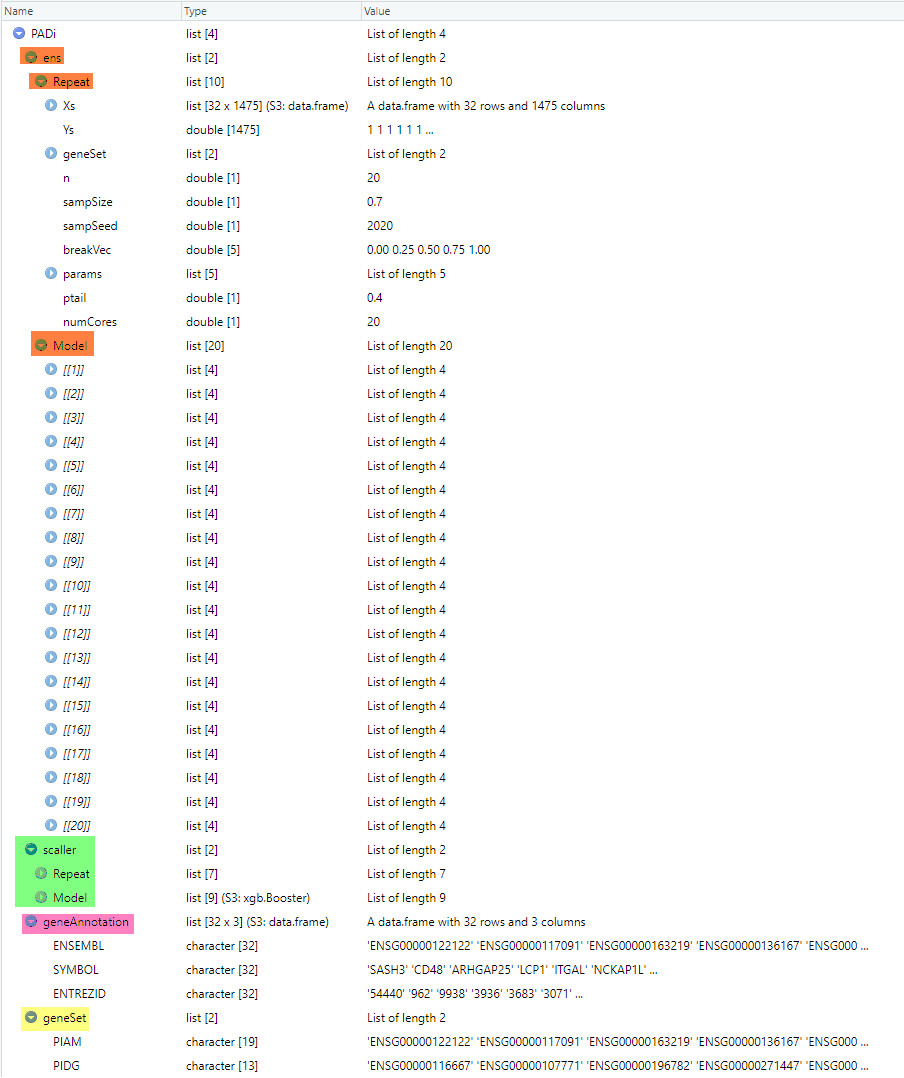
\includegraphics[width=0.9\linewidth]{./fig/GSClassifier-model} 

}

\caption{Details of a GSClassifier model}\label{fig:GSClassifierModel}
\end{figure}

As shown, a typical \passthrough{\lstinline!GSClassifier!} model is consist of four parts (with different colors in the picture):

\begin{itemize}
\tightlist
\item
  \passthrough{\lstinline!1. ens!}:

  \begin{itemize}
  \tightlist
  \item
    \passthrough{\lstinline!Repeat!}: productive parameters of \passthrough{\lstinline!GSClassifier!} models
  \item
    \passthrough{\lstinline!Model!}: \passthrough{\lstinline!GSClassifier!} models. Here, \passthrough{\lstinline!PADi!} had 20 models from different subs of the training cohorts
  \end{itemize}
\item
  \passthrough{\lstinline!2. scaller!}:

  \begin{itemize}
  \tightlist
  \item
    \passthrough{\lstinline!Repeat!}: productive parameters of the \passthrough{\lstinline!scaller!} model, which was used for \passthrough{\lstinline!BestCall!} calling
  \item
    \passthrough{\lstinline!Model!}: the \passthrough{\lstinline!scaller!} model
  \end{itemize}
\item
  \passthrough{\lstinline!3. geneAnnotation!}: a data frame containing gene annotation information
\item
  \passthrough{\lstinline!4. geneSet!}: a list contains several gene sets
\end{itemize}

Thus, you can assemble your model like:

\begin{lstlisting}
model <- list()

# bootstrap models based on the training cohort
model[['ens']] <- <Your model for subtypes calling>

# Scaller model
model[['scaller']] <- <Your scaller for BestCall calling>

# a data frame contarining gene annotation for IDs convertion
model[['geneAnnotation']] <- <Your gene annotation>

# Your gene sets
model[['geneSet']] <- <Your gene sets>

saveRDS(model, 'your-model.rds')
\end{lstlisting}

More tutorials for model establishment, please go to \href{https://github.com/huangwb8/GSClassifier/wiki/Model-establishment}{markdown tutorial} or \href{http://htmlpreview.github.io/?https://raw.githubusercontent.com/wiki/huangwb8/GSClassifier/Model-establishment.html}{html tutorial}.

\hypertarget{submit-models-to-luckymodel-package}{%
\section{Submit models to luckyModel package}\label{submit-models-to-luckymodel-package}}

Considering most users of \passthrough{\lstinline!GSClassifier!} might have no need for lots of models, We divided the model storage feature into an new ensembl package called \href{https://github.com/huangwb8/luckyModel}{\textbf{luckyModel}}. Don't worry, the usage is very easy!

If you want to summit your model, you should apply for a contributor of \passthrough{\lstinline!luckyModel!} first. Then, just send the model (\passthrough{\lstinline!.rds!}) into the \passthrough{\lstinline!inst/extdata/<project>!} path of \passthrough{\lstinline!luckyModel!}. After audit, your branch would be accepted and available for the users.

The name of your model must be the format as following:

\begin{lstlisting}
# <project>
GSClassifier

# <creator>_<model>_v<yyyymmdd>:
HWB_PAD_v20211201.rds
\end{lstlisting}

\hypertarget{repeatablility-of-models}{%
\section{Repeatablility of models}\label{repeatablility-of-models}}

For repeatablility, you had better submit a \passthrough{\lstinline!.zip!} or \passthrough{\lstinline!.tar.gz!} file that containing the information of your model. Here are some suggestions:

\begin{itemize}
\item
  \passthrough{\lstinline!<creator>\_<model>\_v<yyyymmdd>.md!}

  \begin{itemize}
  \item
    \textbf{Destinations}: Why you develop the model
  \item
    \textbf{Design}: The evidence for gene sigatures, et al
  \item
    \textbf{Data sources}: The data for model training and validating, et al
  \item
    \textbf{Applications}: Where to use your model
  \item
    \textbf{Limintations}: Limitation or improvement direction of your model
  \end{itemize}
\item
  \passthrough{\lstinline!<creator>\_<model>\_v<yyyymmdd>.R!}: The code you used for model training and validating.
\item
  \passthrough{\lstinline!Data-of-<creator>\_<model>\_v<yyyymmdd>.rds!} (Optional): Due to huge size of omics data, it's OK for you not to submit the raw data.
\end{itemize}

:cupid: Welcome your contributions!

\hypertarget{gene-annotation}{%
\section{Gene Annotation}\label{gene-annotation}}

For convenience, we provided a general gene annotation dataset for different genomics:

\begin{lstlisting}[language=R]
gga <- readRDS(system.file("extdata", "general-gene-annotation.rds", package = "GSClassifier"))
names(gga)
# [1] "hg38" "hg19" "mm10"
\end{lstlisting}

I believe they're enough for routine medicine studies.

Here, take a look at \passthrough{\lstinline!hg38!}:

\begin{lstlisting}[language=R]
hg38 <- gga$hg38
head(hg38)
#           ENSEMBL       SYMBOL  ENTREZID
# 1 ENSG00000223972      DDX11L1 100287102
# 3 ENSG00000227232       WASH7P      <NA>
# 4 ENSG00000278267    MIR6859-1 102466751
# 5 ENSG00000243485 RP11-34P13.3      <NA>
# 6 ENSG00000284332    MIR1302-2 100302278
# 7 ENSG00000237613      FAM138A    645520
\end{lstlisting}

With this kind of data, it's simple to customize your own gene annotation (take \passthrough{\lstinline!PADi!} as examples):

\begin{lstlisting}[language=R]

tGene <- as.character(unlist(PADi$geneSet))
geneAnnotation <- hg38[hg38$ENSEMBL %in% tGene, ]
dim(geneAnnotation)
# [1] 32  3
\end{lstlisting}

Have a check:

\begin{lstlisting}[language=R]
head(geneAnnotation)
#              ENSEMBL SYMBOL ENTREZID
# 353  ENSG00000171608 PIK3CD     5293
# 1169 ENSG00000134686   PHC2     1912
# 2892 ENSG00000134247 PTGFRN     5738
# 3855 ENSG00000117090 SLAMF1     6504
# 3858 ENSG00000117091   CD48      962
# 4043 ENSG00000198821  CD247      919
\end{lstlisting}

This \passthrough{\lstinline!geneAnnotation!} could be the \passthrough{\lstinline!model[['geneAnnotation']]!}.

Also, we use a function called \passthrough{\lstinline!convert!} to do gene ID convertion.

\begin{lstlisting}[language=R]
luckyBase::convert(c('GAPDH','TP53'), 'SYMBOL', 'ENSEMBL', hg38)
# [1] "ENSG00000111640" "ENSG00000141510"
\end{lstlisting}

Note: the \passthrough{\lstinline!luckyBase!} package integrates lots of useful tiny functions, you could explore it sometimes.

\hypertarget{references}{%
\chapter*{References}\label{references}}
\addcontentsline{toc}{chapter}{References}

\hypertarget{refs}{}
\begin{CSLReferences}{0}{0}
\leavevmode\vadjust pre{\hypertarget{ref-RN160}{}}%
1. Thorsson V, Gibbs DL, Brown SD, et al. \href{https://doi.org/10.1016/j.immuni.2018.03.023}{The immune landscape of cancer}. Immunity 2018; 48:812--830 e14

\leavevmode\vadjust pre{\hypertarget{ref-RN315}{}}%
2. Gibbs DL. Robust classification of immune subtypes in cancer. 2020;

\leavevmode\vadjust pre{\hypertarget{ref-RN345}{}}%
3. Chen T, He T, Benesty M, et al. Xgboost: Extreme gradient boosting. 2015; 1:1--4

\leavevmode\vadjust pre{\hypertarget{ref-RN267}{}}%
4. Geman D, d'Avignon C, Naiman DQ, et al. \href{https://doi.org/10.2202/1544-6115.1071}{Classifying gene expression profiles from pairwise mRNA comparisons}. Stat Appl Genet Mol Biol 2004; 3:Article19

\leavevmode\vadjust pre{\hypertarget{ref-RN265}{}}%
5. Zhao H, Logothetis CJ, Gorlov IP. \href{https://doi.org/10.1038/pcan.2010.9}{Usefulness of the top-scoring pairs of genes for prediction of prostate cancer progression}. Prostate Cancer Prostatic Dis 2010; 13:252--9

\leavevmode\vadjust pre{\hypertarget{ref-RN266}{}}%
6. Youssef YM, White NM, Grigull J, et al. \href{https://doi.org/10.1016/j.eururo.2011.01.004}{Accurate molecular classification of kidney cancer subtypes using microRNA signature}. Eur Urol 2011; 59:721--30

\leavevmode\vadjust pre{\hypertarget{ref-RN261}{}}%
7. Auslander N, Zhang G, Lee JS, et al. \href{https://doi.org/10.1038/s41591-018-0157-9}{Robust prediction of response to immune checkpoint blockade therapy in metastatic melanoma}. Nat Med 2018; 24:1545--1549

\leavevmode\vadjust pre{\hypertarget{ref-RN387}{}}%
8. Troyanskaya O, Cantor M, Sherlock G, et al. \href{https://doi.org/10.1093/bioinformatics/17.6.520}{Missing value estimation methods for DNA microarrays}. Bioinformatics 2001; 17:520--5

\leavevmode\vadjust pre{\hypertarget{ref-RN389}{}}%
9. Arbeitman MN, Furlong EE, Imam F, et al. \href{https://doi.org/10.1126/science.1072152}{Gene expression during the life cycle of drosophila melanogaster}. Science 2002; 297:2270--5

\leavevmode\vadjust pre{\hypertarget{ref-RN382}{}}%
10. Zhu X, Wang J, Sun B, et al. \href{https://doi.org/10.1186/s12859-021-04109-4}{An efficient ensemble method for missing value imputation in microarray gene expression data}. BMC Bioinformatics 2021; 22:188

\leavevmode\vadjust pre{\hypertarget{ref-RN392}{}}%
11. Lin W-C, Tsai C-F. Missing value imputation: A review and analysis of the literature (2006--2017). 2020; 53:1487--1509

\leavevmode\vadjust pre{\hypertarget{ref-RN386}{}}%
12. Hasan MK, Alam MA, Roy S, et al. Missing value imputation affects the performance of machine learning: A review and analysis of the literature (2010--2021). Informatics in Medicine Unlocked 2021; 27:100799

\leavevmode\vadjust pre{\hypertarget{ref-RN384}{}}%
13. Wang A, Yang J, An N. Regularized sparse modelling for microarray missing value estimation. 2021; 9:16899--16913

\leavevmode\vadjust pre{\hypertarget{ref-xgboost}{}}%
14. Chen T, He T, Benesty M, et al. \href{https://CRAN.R-project.org/package=xgboost}{Xgboost: Extreme gradient boosting}. 2022;

\leavevmode\vadjust pre{\hypertarget{ref-pROC}{}}%
15. Robin X, Turck N, Hainard A, et al. pROC: An open-source package for r and s+ to analyze and compare ROC curves. BMC Bioinformatics 2011; 12:77

\leavevmode\vadjust pre{\hypertarget{ref-RN369}{}}%
16. Zhu S, Kong W, Zhu J, et al. \href{https://doi.org/10.1093/bib/bbac344}{The genetic algorithm-aided three-stage ensemble learning method identified a robust survival risk score in patients with glioma}. Brief Bioinform 2022;

\leavevmode\vadjust pre{\hypertarget{ref-RN367}{}}%
17. Tong M, Zheng W, Li H, et al. \href{https://doi.org/10.1038/oncsis.2016.51}{Multi-omics landscapes of colorectal cancer subtypes discriminated by an individualized prognostic signature for 5-fluorouracil-based chemotherapy}. Oncogenesis 2016; 5:e242

\leavevmode\vadjust pre{\hypertarget{ref-RN368}{}}%
18. Qi L, Li Y, Qin Y, et al. \href{https://doi.org/10.1038/bjc.2016.370}{An individualised signature for predicting response with concordant survival benefit for lung adenocarcinoma patients receiving platinum-based chemotherapy}. Br J Cancer 2016; 115:1513--1519

\leavevmode\vadjust pre{\hypertarget{ref-RN364}{}}%
19. Huang H, Zou Y, Zhang H, et al. \href{https://doi.org/10.1016/j.trsl.2020.02.004}{A qualitative transcriptional prognostic signature for patients with stage i-II pancreatic ductal adenocarcinoma}. Transl Res 2020; 219:30--44

\leavevmode\vadjust pre{\hypertarget{ref-RN363}{}}%
20. Zheng H, Song K, Fu Y, et al. \href{https://doi.org/10.1093/bib/bbz174}{An absolute human stemness index associated with oncogenic dedifferentiation}. Brief Bioinform 2021; 22:2151--2160

\leavevmode\vadjust pre{\hypertarget{ref-RN362}{}}%
21. Kong W, He L, Zhu J, et al. \href{https://doi.org/10.1038/s41375-022-01662-6}{An immunity and pyroptosis gene-pair signature predicts overall survival in acute myeloid leukemia}. Leukemia 2022;

\leavevmode\vadjust pre{\hypertarget{ref-RN366}{}}%
22. Liu K, Geng Y, Wang L, et al. \href{https://doi.org/10.1002/1878-0261.13279}{Systematic exploration of the underlying mechanism of gemcitabine resistance in pancreatic adenocarcinoma}. Mol Oncol 2022; 16:3034--3051

\leavevmode\vadjust pre{\hypertarget{ref-RN365}{}}%
23. Zheng H, Xie J, Song K, et al. \href{https://doi.org/10.1186/s13287-022-02803-5}{StemSC: A cross-dataset human stemness index for single-cell samples}. Stem Cell Res Ther 2022; 13:115

\end{CSLReferences}

\end{document}
